\chapter{Polyhedral Relations}\label{sec:gpa}

We now turn to a combinatorially richer class of objects: polyhedra and polyhedral
cones. These are the fundamental geometric structures underlying linear
programming, and they admit a categorical treatment entirely analogous to
the one developed for linear and affine relations.
The key difference is that
composition here is governed by Fourier-Motzkin Elimination (FME): projecting a polyhedron onto a subspace is
precisely variable elimination, and it is this operation that categorical
composition will simulate diagrammatically.

The theory developed here remains
within the category of binary relations, since morphisms are still indicator functions
of subsets of $\mathbb{R}^n \times \mathbb{R}^m$, encoding feasibility
constraints rather than objective functions. In this sense, $\mathbf{GPA}$
does not yet enter the weighted relational world, and so is not yet able to express more meaningful
optimization problems. This is nonetheless a critical step in the development.
Axiomatizing linear inequality constraints diagrammatically,  $\mathbf{GPA}$ provides
the Symmetric Monoidal Inequality Theory (SMIT)~\cite{bonchi2021polyhedral}  that will
serve as the structural foundation for our final contribution,  $\mathbf{GLP}$,
where these constraints are combined with a linear objective to form full parametric linear programs.


In what follows we describe and show the complete theory of polyhedral relations and polyhedral cones.
Just as $\mathbf{AffRel}$ captured affine space as morphisms, the categories $\mathbf{PCRel}$ and
$\mathbf{PolyRel}$ capture polyhedral cones and polyhedra as morphisms,
with relational composition playing the role of variable elimination.

\section{Semantics: the prop \texorpdfstring{$\mathbf{PCRel}$}{PCRel} of polyhedral cones}

We begin by recalling the standard definitions of polyhedral cones and the corresponding semantic category.

\begin{definition}\label{def:pcform}
	A set $C \subseteq \mathbb{R}^n$ is called a \emph{polyhedral cone} if
	there exists a matrix $A \in \mathbb{R}^{m \times n}$ such that
	\[
		C = \{x \in \mathbb{R}^n \mid Ax \ge 0\}.
	\]
\end{definition}

\begin{definition}[The prop $\mathbf{PCRel}$ of polyhedral cones]
	Let $k$ be an ordered field, in this case the real numbers. The prop
	$\mathbf{PCRel}_k$ is defined as follows:
	\begin{itemize}
		\item Objects are natural numbers $n \in \mathbb{N}$, interpreted
		      as the space $k^n$.
		\item A morphism $n \to m$ is a polyhedral cone
		      $R \subseteq k^n \times k^m$
		      for which there exist $p \in \mathbb{N}$ and
		      $A \in k^{p \times (n+m)}$ such that
		      \[
			      R = \left\{ (x,y) \in k^n \times k^m \;\middle|\;
			      A \begin{pmatrix} x \\ y \end{pmatrix} \ge 0 \right\}.
		      \]
		\item Composition is relational composition.
		\item The monoidal product on objects is addition $n \otimes m := n+m$,
		      and on morphisms is the Cartesian product.
	\end{itemize}
\end{definition}

Observe that in comparison with the previous categories of \textbf{AffRel},
this category is way more general although it does not completely encode the notion of Affine Spaces. However,
it does introduce to us a somewhat unorthodox notion of conical polyhedral relations. That is,
the fact that two elements $x,y$ may be related to one another by a relation $R$ such that the set of all pairs $xRy$
form a polyhedral cone.
Although this description remains very set-theoretically,
it starts to flirt with the idea of $x$ and $y$ being apparted from a specific class of maps.
More precisely, instead of thinking of the whole geometry of polyhedral cones,
one may think of the pairs $(x,y)$ such that $Ax \ge By$ for some $A$ and $B$ fully defined by the relation $R$.

\section{Syntax: the algebra \texorpdfstring{$\mathbf{GPA}_{\rtop}$}{GPA}}

\begin{definition}[Graphical Polyhedral Algebra]\label{def:gpa}
	We call $\mathbf{GPA}$ the SMT generated by extending $\mathbf{GAA}$
	with the following generator and its semantics:
	\begin{figure}[H]
        \centering
        \begin{tikzpicture}[axpic]
            \node at (0.0,0.5) {$\llbracket$};
            \pic (g1) at (0.600,0.500) {ge};
            \node at (1.2,0.5) {$\rrbracket$};
        \end{tikzpicture}
        \begin{tikzpicture}[axpic]
            \node{$= \{ (x,y) | x,y \in k, x \ge y\}$};
        \end{tikzpicture}
	\end{figure}
	along with the following additional equations:
	\begin{figure}[H]
		\centering
		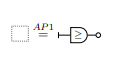
\includegraphics[width=0.2\linewidth]{images/GPA/AffineAxiom.png}
	\end{figure}
	% Axioms of GPA, in addition to those of GAA: the inequality generator is a
% lax (co)monoid morphism (P1-P4), interacts with scalars by sign (P5, P6),
% and is antisymmetric, spider-like and directed.
\begin{center}\begin{tabular}{r c c c}
  (P1) & \begin{tikzpicture}[axpic]
      \pic (g1) at (0.500,0.500) {ge};
      \pic (g2) at (1.750,0.500) {copy};
      \draw (g1-out-0) to[out=0,in=180] (g2-in-0);
  \end{tikzpicture}
  & \;\begin{tikzpicture}[axpic]\node{$\subseteq$};\end{tikzpicture}\;
  & \begin{tikzpicture}[axpic]
      \pic (g1) at (0.500,0.500) {copy};
      \pic (g2) at (1.750,1.000) {ge};
      \pic (g3) at (1.750,0.000) {ge};
      \draw (g1-out-0) to[out=0,in=180] (g2-in-0);
      \draw (g1-out-1) to[out=0,in=180] (g3-in-0);
  \end{tikzpicture} \\[1mm]
  \diagrow{(P2)}{
      \pic (g1) at (0.500,0.500) {multiplication};
      \pic (g2) at (1.750,0.500) {ge};
      \draw (g1-out-0) to[out=0,in=180] (g2-in-0);
  }{
      \pic (g1) at (0.500,1.000) {ge};
      \pic (g2) at (0.500,0.000) {ge};
      \pic (g3) at (1.750,0.500) {multiplication};
      \draw (g1-out-0) to[out=0,in=180] (g3-in-0);
      \draw (g2-out-0) to[out=0,in=180] (g3-in-1);
  }
  \diagrow{(P3)}{
      \pic (g1) at (0.500,0.500) {ge};
      \pic (g2) at (1.750,0.500) {discard};
      \draw (g1-out-0) -- (g2-in-0);
  }{
      \pic (g1) at (0.500,0.500) {discard};
      \draw (-0.250,0.500) -- (g1-in-0);
  }
  (P4) & \begin{tikzpicture}[axpic]
      \pic (g1) at (0.500,0.500) {zero};
      \draw (g1-out-0) -- (1.250,0.500);
  \end{tikzpicture}
  & \;\begin{tikzpicture}[axpic]\node{$\subseteq$};\end{tikzpicture}\;
  & \begin{tikzpicture}[axpic]
      \pic (g1) at (0.500,0.500) {zero};
      \pic (g2) at (1.750,0.500) {ge};
      \draw (g1-out-0) to[out=0,in=180] (g2-in-0);
  \end{tikzpicture} \\[1mm]
\end{tabular}\end{center}

\begin{center}\begin{tabular}{r c c c}
  \diagrow{(P5) \ $k>0$}{
      \pic[val=k] (g1) at (0.500,0.500) {scalar};
      \pic (g2) at (1.750,0.500) {ge};
      \draw (g1-out-0) to[out=0,in=180] (g2-in-0);
  }{
      \pic (g1) at (0.500,0.500) {ge};
      \pic[val=k] (g2) at (1.750,0.500) {scalar};
      \draw (g1-out-0) to[out=0,in=180] (g2-in-0);
  }
  \diagrow{(P6) \ $k<0$}{
      \pic[val=k] (g1) at (0.500,0.500) {scalar};
      \pic (g2) at (1.750,0.500) {ge};
      \draw (g1-out-0) to[out=0,in=180] (g2-in-0);
  }{
      \pic (g1) at (0.500,0.500) {coge};
      \pic[val=k] (g2) at (1.750,0.500) {scalar};
      \draw (g1-out-0) to[out=0,in=180] (g2-in-0);
  }
\end{tabular}\end{center}

\begin{center}\begin{tabular}{r c c c}
  (antisym) & \begin{tikzpicture}[axpic]
      \pic (g1) at (0.500,0.500) {copy};
      \pic (g2) at (1.750,1.000) {ge};
      \pic (g3) at (1.750,0.000) {coge};
      \pic (g4) at (3.000,0.500) {cocopy};
      \draw (g1-out-0) to[out=0,in=180] (g2-in-0);
      \draw (g1-out-1) to[out=0,in=180] (g3-in-0);
      \draw (g2-out-0) to[out=0,in=180] (g4-in-0);
      \draw (g3-out-0) to[out=0,in=180] (g4-in-1);
  \end{tikzpicture}
  & \;\begin{tikzpicture}[axpic]\node{$\subseteq$};\end{tikzpicture}\;
  & \begin{tikzpicture}[axpic]
      \draw (0.000,0.500) -- (1.250,0.500);
  \end{tikzpicture} \\[2mm]
  \diagrow{(spider)}{
      \pic (g1) at (0.500,1.000) {ge};
      \pic (g2) at (0.500,0.000) {ge};
      \pic (c1) at (1.750,0.500) {cocopy};
      \pic (c2) at (3.000,0.500) {copy};
      \pic (h1) at (4.250,1.000) {ge};
      \pic (h2) at (4.250,0.000) {ge};
      \draw (g1-out-0) to[out=0,in=180] (c1-in-0);
      \draw (g2-out-0) to[out=0,in=180] (c1-in-1);
      \draw (c1-out-0) -- (c2-in-0);
      \draw (c2-out-0) to[out=0,in=180] (h1-in-0);
      \draw (c2-out-1) to[out=0,in=180] (h2-in-0);
  }{
      \pic (c1) at (0.500,1.500) {copy};
      \pic (c2) at (0.500,-0.500) {copy};
      \pic (g11) at (2.000,2.000) {ge};
      \pic (g12) at (2.000,1.000) {ge};
      \pic (g21) at (2.000,0.000) {ge};
      \pic (g22) at (2.000,-1.000) {ge};
      \pic (d1) at (3.750,1.500) {cocopy};
      \pic (d2) at (3.750,-0.500) {cocopy};
      \draw (c1-out-0) to[out=0,in=180] (g11-in-0);
      \draw (c1-out-1) to[out=0,in=180] (g12-in-0);
      \draw (c2-out-0) to[out=0,in=180] (g21-in-0);
      \draw (c2-out-1) to[out=0,in=180] (g22-in-0);
      \draw (g11-out-0) to[out=0,in=180] (d1-in-0);
      \draw (g21-out-0) to[out=0,in=180] (d1-in-1);
      \draw (g12-out-0) to[out=0,in=180] (d2-in-0);
      \draw (g22-out-0) to[out=0,in=180] (d2-in-1);
  }
  \diagrow{(direction)}{
      \pic (g1) at (0.500,0.500) {coge};
      \pic (g2) at (1.500,0.500) {ge};
      \draw (g1-out-0) -- (g2-in-0);
  }{
      \pic (g1) at (0.500,0.500) {discard};
      \pic (g2) at (1.750,0.500) {codiscard};
      \draw (-0.250,0.500) -- (g1-in-0);
      \draw (g2-out-0) -- (2.500,0.500);
  }
\end{tabular}\end{center}

\end{definition}

\begin{definition}[Graphical Polyhedral Cones Algebra]
	We call $\mathbf{GPA}_{\rtop}$ the SMT generated by $\mathbf{GPA}$
	but excluding the affine generator $\rtop$ and its associated
	equations. This fragment axiomatises polyhedral cones, where no
	translation is present.
\end{definition}

\begin{definition}[The Free Categories of Polyhedral Diagrams]
	We call $\mathrm{FreeP}_{\mathbf{GPA}}$ the PROP freely generated
	by $\mathbf{GPA}$, and $\mathrm{FreeP}_{\mathbf{GPA}_{\rtop}}$ the
	PROP freely generated by $\mathbf{GPA}_{\rtop}$.
\end{definition}


\section{The order structure of the inequality generator}\label{sec:gpa-rules}

The central computational primitive for reasoning inside this algebra is
Fourier--Motzkin Elimination, which projects a polyhedral cone onto a
lower-dimensional space by eliminating one variable at a time.

It is worth being explicit about what that algorithm actually does to a system
$Ax\ge0$, because it fixes exactly which diagrammatic rules we have to
establish first. To eliminate a variable $t$, the algorithm divides each row
containing $t$ by its coefficient, so that the row becomes a bound on $t$;
it records whether the bound is an upper or a lower one, according to the sign
of that coefficient; and it then replaces the whole collection of bounds by
one inequality for each upper--lower pair. Three moves, therefore: rescaling a
row, moving a term across a sum, and merging bounds pairwise. Two of them are
axioms of Definition~\ref{def:gpa}; this section supplies the third and the
order laws the axioms omit, and Section~\ref{sec:gpa-fme} assembles them into
the elimination itself.

Rescaling and sign are given outright by (P5) and (P6), and the pairwise merge
by (spider). What the axioms do not state, and what we need first, is that
$\inlinegen{ge}$ deserves its name: reflexivity and transitivity are not among
them, and antisymmetry is postulated only as the inclusion
$\subseteq$.

\begin{lemma}[The generator is an order]\label{lem:order}
	In $\mathbf{GPA}_{\rtop}$ the generator $\inlinegen{ge}$ is reflexive,
	transitive and antisymmetric.
\end{lemma}

\begin{proof}
	Transitivity is (spider) with one input fed by the black unit and one
	output discarded, the plugs being absorbed by (P3) and the black
	(co)unit laws:
	% Transitivity of the inequality generator: the (spider) axiom with one input
% fed by the black unit and one output discarded.
\begin{center}
    \begin{tikzpicture}[axpic]
        \pic (g1) at (0.500,0.500) {ge};
        \pic (g2) at (1.750,0.500) {ge};
        \draw (g1-out-0) to[out=0,in=180] (g2-in-0);
    \end{tikzpicture} \\
    \vspace{3mm}

    \;\begin{tikzpicture}[axpic]\node{$\overset{(\text{unit})}{=}$};\end{tikzpicture}\;
    \begin{tikzpicture}[axpic]
        \pic (u)  at (0.400,0.000) {codiscard};
        \pic (g1) at (1.900,1.000) {ge};
        \pic (g2) at (1.900,0.000) {ge};
        \pic (c1) at (3.150,0.500) {cocopy};
        \pic (c2) at (4.400,0.500) {copy};
        \pic (h1) at (5.650,1.000) {ge};
        \pic (h2) at (5.650,0.000) {ge};
        \pic (d)  at (6.900,0.000) {discard};
        \draw (0.900,1.000) -- (g1-in-0);
        \draw (u-out-0) -- (g2-in-0);
        \draw (g1-out-0) to[out=0,in=180] (c1-in-0);
        \draw (g2-out-0) to[out=0,in=180] (c1-in-1);
        \draw (c1-out-0) -- (c2-in-0);
        \draw (c2-out-0) to[out=0,in=180] (h1-in-0);
        \draw (c2-out-1) to[out=0,in=180] (h2-in-0);
        \draw (h1-out-0) -- (6.900,1.000);
        \draw (h2-out-0) -- (d-in-0);
    \end{tikzpicture} \\
    \vspace{3mm}

    \;\begin{tikzpicture}[axpic]\node{$\overset{(\text{spider})}{=}$};\end{tikzpicture}\;
    \begin{tikzpicture}[axpic]
        \pic (u)   at (0.400,-0.500) {codiscard};
        \pic (c1)  at (1.400,1.500) {copy};
        \pic (c2)  at (1.400,-0.500) {copy};
        \pic (g11) at (2.900,2.000) {ge};
        \pic (g12) at (2.900,1.000) {ge};
        \pic (g21) at (2.900,0.000) {ge};
        \pic (g22) at (2.900,-1.000) {ge};
        \pic (d1)  at (4.650,1.500) {cocopy};
        \pic (d2)  at (4.650,-0.500) {cocopy};
        \pic (dd)  at (5.900,-0.500) {discard};
        \draw (0.400,1.500) -- (c1-in-0);
        \draw (u-out-0) -- (c2-in-0);
        \draw (c1-out-0) to[out=0,in=180] (g11-in-0);
        \draw (c1-out-1) to[out=0,in=180] (g12-in-0);
        \draw (c2-out-0) to[out=0,in=180] (g21-in-0);
        \draw (c2-out-1) to[out=0,in=180] (g22-in-0);
        \draw (g11-out-0) to[out=0,in=180] (d1-in-0);
        \draw (g21-out-0) to[out=0,in=180] (d1-in-1);
        \draw (g12-out-0) to[out=0,in=180] (d2-in-0);
        \draw (g22-out-0) to[out=0,in=180] (d2-in-1);
        \draw (d1-out-0) -- (5.900,1.500);
        \draw (d2-out-0) -- (dd-in-0);
    \end{tikzpicture} \\
    \vspace{3mm}

    \;\begin{tikzpicture}[axpic]\node{$\overset{(P3),(\text{unit})}{=}$};\end{tikzpicture}\;
    \begin{tikzpicture}[axpic]
        \pic (g1) at (0.500,0.500) {ge};
    \end{tikzpicture}
\end{center}


	\noindent Reflexivity:
	\begin{center}
		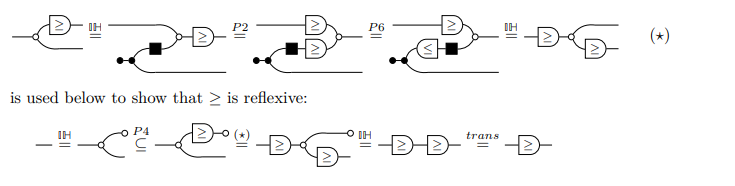
\includegraphics[width=\linewidth]{images/GPA/reflexivity.png}
	\end{center}

	\noindent Antisymmetry, the converse of the inclusion (antisym):
	\begin{center}
		\begin{tikzpicture}
    \node{(1)};
\end{tikzpicture}\;
\begin{tikzpicture}[axpic]
  \begin{scope}[shift={(0.000,0.500)}]
  \pic (g1) at (0.500,0.500) {copy};
  \end{scope}
  \begin{scope}[shift={(1.250,0.000)}]
  \begin{scope}[shift={(0.000,1.000)}]
  \pic (g2) at (0.500,0.500) {ge};
  \end{scope}
  \pic (g3) at (0.500,0.500) {coge};
  \end{scope}
  \draw (g1-out-0) to[out=0,in=180] (g2-in-0);
  \draw (g1-out-1) to[out=0,in=180] (g3-in-0);
  \begin{scope}[shift={(2.500,0.500)}]
  \pic (g4) at (0.500,0.500) {cocopy};
  \end{scope}
  \draw (g2-out-0) to[out=0,in=180] (g4-in-0);
  \draw (g3-out-0) to[out=0,in=180] (g4-in-1);
\end{tikzpicture}
\;\begin{tikzpicture}[axpic]\node{$\subseteq$};\end{tikzpicture}\;
\begin{tikzpicture}[axpic]
  \coordinate (id_in_1) at (0,0.500);
  \coordinate (id_out_2) at (1.000,0.500);
  \draw (id_in_1) -- (id_out_2);
\end{tikzpicture}

\vspace{5mm}

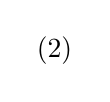
\begin{tikzpicture}
    \node{(2)};
\end{tikzpicture}\;
\begin{tikzpicture}[axpic]
  \coordinate (id_in_1) at (0,0.500);
  \coordinate (id_out_2) at (1.000,0.500);
  \draw (id_in_1) -- (id_out_2);
\end{tikzpicture}
\;\begin{tikzpicture}[axpic]\node{$=$};\end{tikzpicture}\;
\begin{tikzpicture}[axpic]
  \pic (g1) at (0.500,0.500) {copy};
  \begin{scope}[shift={(1.250,0.000)}]
  \pic (g2) at (0.500,0.500) {cocopy};
  \end{scope}
  \draw (g1-out-0) to[out=0,in=180] (g2-in-0);
  \draw (g1-out-1) to[out=0,in=180] (g2-in-1);
\end{tikzpicture}
\;\begin{tikzpicture}[axpic]\node{$\subseteq$};\end{tikzpicture}\;
\begin{tikzpicture}[axpic]
  \begin{scope}[shift={(0.000,0.500)}]
  \pic (g1) at (0.500,0.500) {copy};
  \end{scope}
  \begin{scope}[shift={(1.250,0.000)}]
  \begin{scope}[shift={(0.000,1.000)}]
  \pic (g2) at (0.500,0.500) {ge};
  \end{scope}
  \pic (g3) at (0.500,0.500) {coge};
  \end{scope}
  \draw (g1-out-0) to[out=0,in=180] (g2-in-0);
  \draw (g1-out-1) to[out=0,in=180] (g3-in-0);
  \begin{scope}[shift={(2.500,0.500)}]
  \pic (g4) at (0.500,0.500) {cocopy};
  \end{scope}
  \draw (g2-out-0) to[out=0,in=180] (g4-in-0);
  \draw (g3-out-0) to[out=0,in=180] (g4-in-1);
\end{tikzpicture}

\vspace{5mm}
\;\begin{tikzpicture}[axpic]\node{$(1)\wedge(2)\implies$};\end{tikzpicture}\;
\begin{tikzpicture}[axpic]
  \coordinate (id_in_1) at (0,0.500);
  \coordinate (id_out_2) at (1.000,0.500);
  \draw (id_in_1) -- (id_out_2);
\end{tikzpicture}
\;\begin{tikzpicture}[axpic]\node{$=$};\end{tikzpicture}\;
\begin{tikzpicture}[axpic]
  \begin{scope}[shift={(0.000,0.500)}]
  \pic (g1) at (0.500,0.500) {copy};
  \end{scope}
  \begin{scope}[shift={(1.250,0.000)}]
  \begin{scope}[shift={(0.000,1.000)}]
  \pic (g2) at (0.500,0.500) {ge};
  \end{scope}
  \pic (g3) at (0.500,0.500) {coge};
  \end{scope}
  \draw (g1-out-0) to[out=0,in=180] (g2-in-0);
  \draw (g1-out-1) to[out=0,in=180] (g3-in-0);
  \begin{scope}[shift={(2.500,0.500)}]
  \pic (g4) at (0.500,0.500) {cocopy};
  \end{scope}
  \draw (g2-out-0) to[out=0,in=180] (g4-in-0);
  \draw (g3-out-0) to[out=0,in=180] (g4-in-1);
\end{tikzpicture}

	\end{center}
\end{proof}

Since $\inlinegen{coge}$ is $\inlinegen{ge}$ with an antipode on each side, by
(P6) at $k=-1$, every axiom comes in a mirrored version, and we use both
without further comment.

The move the axioms leave implicit is the transport of a term across a sum: it
is the step that turns a row of a system into a bound on a single variable,
and it is the content of the next lemma.

\begin{lemma}[Cap form]\label{lem:capform}
	In $\mathbf{GPA}_{\rtop}$,
	% An inequality may be moved across a white sum; and a row s+u >= 0 is the
% cap form of s >= -u.
\begin{center}
    \begin{tikzpicture}[axpic]
        \node at (-1.0,0.5) {$(C1)$};
        \pic (g1) at (0.500,1.000) {ge};
        \pic (g2) at (1.750,0.500) {multiplication};
        \coordinate (id_in_1)  at (0.000,0.000);
        \coordinate (id_out_1) at (1.250,0.000);
        \draw (id_in_1) -- (id_out_1);
        \draw (g1-out-0) to[out=0,in=180] (g2-in-0);
        \draw (id_out_1) to[out=0,in=180] (g2-in-1);
    \end{tikzpicture}
    \;\begin{tikzpicture}[axpic]\node{$=$};\end{tikzpicture}\;
    \begin{tikzpicture}[axpic]
        \pic (g1) at (0.500,0.500) {multiplication};
        \pic (g2) at (1.750,0.500) {ge};
        \draw (g1-out-0) to[out=0,in=180] (g2-in-0);
    \end{tikzpicture}
    \;\begin{tikzpicture}[axpic]\node{$=$};\end{tikzpicture}\;
    \begin{tikzpicture}[axpic]
        \pic (g1) at (0.500,0.000) {ge};
        \pic (g2) at (1.750,0.500) {multiplication};
        \coordinate (id_in_1)  at (0.000,1.000);
        \coordinate (id_out_1) at (1.250,1.000);
        \draw (id_in_1) -- (id_out_1);
        \draw (id_out_1) to[out=0,in=180] (g2-in-0);
        \draw (g1-out-0) to[out=0,in=180] (g2-in-1);
    \end{tikzpicture} \\
    \vspace{4mm}

    \begin{tikzpicture}[axpic]
        \node at (-1.0,0.5) {$(C2)$};
        \pic (g1) at (0.500,0.500) {multiplication};
        \pic (g2) at (1.750,0.500) {ge};
        \pic (g3) at (3.000,0.500) {cozero};
        \draw (g1-out-0) to[out=0,in=180] (g2-in-0);
        \draw (g2-out-0) to[out=0,in=180] (g3-in-0);
    \end{tikzpicture}
    \;\begin{tikzpicture}[axpic]\node{$=$};\end{tikzpicture}\;
    \begin{tikzpicture}[axpic]
        \pic (g1) at (0.500,1.000) {ge};
        \pic (g2) at (0.500,0.000) {antipode};
        \draw (g1-out-0) -- (1.600,1.000) arc (90:-90:0.500) -- (g2-out-0);
    \end{tikzpicture}
\end{center}

\end{lemma}

The first chain reads $x+u\ge v$ iff $v-u\le x$: an inequality may be applied
before or after a sum indifferently. The second reads $s+u\ge0$ iff
$s\ge-u$, and it is the form we shall use: the diagram
$(\inlinegen{ge}\oplus\mathrm{id});\varepsilon$, whose denotation is
$\{(\ell,r)\mid \ell\ge r\}$, we call the \emph{cap form} of $\ell\ge r$, so
that a row $s+u\ge0$ of a system is the cap form of the bound $s\ge-u$.

\begin{proof}
	Bending the second input of the white sum to an output is a bijection on
	hom-sets, so the first equation may be compared in bent form; the third
	follows by commutativity of the sum. Closing the bent leg with a white
	cozero then gives the second equation.
	% Proof of (C1): an inequality may be applied before or after a white sum.
% Proof of (C2): closing the sum with a white cozero gives the cap form.
% Broken over lines to fit the text block; all diagrams share the
% convention that the sum sits at y=1.0, its top leg at y=1.5 and its bottom
% leg at y=0.5, so that legs meet the sum without kinks.
\begin{center}
    \begin{tikzpicture}[axpic]\node{$(C1)$};\end{tikzpicture}\;
    \begin{tikzpicture}[axpic]
        \pic (g1) at (0.500,1.500) {ge};
        \pic (a1) at (1.750,1.000) {multiplication};
        \coordinate (id_in_1)  at (0.000,0.500);
        \coordinate (id_out_1) at (1.000,0.500);
        \draw (id_in_1) -- (id_out_1);
        \draw (g1-out-0) -- (a1-in-0);
        \draw (id_out_1) -- (a1-in-1);
        \draw (a1-out-0) -- (2.750,1.000);
    \end{tikzpicture}
    \;\begin{tikzpicture}[axpic]\node{$=$};\end{tikzpicture}\;
    \begin{tikzpicture}[axpic]
        \pic (g1) at (0.500,1.500) {ge};
        \pic (g2) at (1.750,1.500) {ge};
        \pic (a1) at (3.000,1.000) {multiplication};
        \coordinate (id_in_1)  at (0.000,0.500);
        \coordinate (id_out_1) at (2.250,0.500);
        \draw (id_in_1) -- (id_out_1);
        \draw (g1-out-0) -- (g2-in-0);
        \draw (g2-out-0) -- (a1-in-0);
        \draw (id_out_1) -- (a1-in-1);
        \draw (a1-out-0) -- (4.000,1.000);
    \end{tikzpicture}
    \;\begin{tikzpicture}[axpic]\node{$=$};\end{tikzpicture}\;
    \begin{tikzpicture}[axpic]
        \pic (g1) at (0.500,1.500) {ge};
        \pic (g2) at (0.500,0.500) {ge};
        \pic (a1) at (1.750,1.000) {multiplication};
        \pic (g3) at (3.000,1.000) {ge};
        \draw (g1-out-0) -- (a1-in-0);
        \draw (g2-out-0) -- (a1-in-1);
        \draw (a1-out-0) -- (g3-in-0);
        \draw (g3-out-0) -- (3.500,1.000);
    \end{tikzpicture} \\
    \vspace{3mm}

    \;\begin{tikzpicture}[axpic]\node{$=$};\end{tikzpicture}\;
    \begin{tikzpicture}[axpic]
        \pic (a1) at (0.750,1.000) {multiplication};
        \pic (g1) at (2.000,1.000) {ge};
        \pic (g2) at (3.250,1.000) {ge};
        \draw (a1-out-0) -- (g1-in-0);
        \draw (g1-out-0) -- (g2-in-0);
        \draw (g2-out-0) -- (3.750,1.000);
    \end{tikzpicture}
    \;\begin{tikzpicture}[axpic]\node{$=$};\end{tikzpicture}\;
    \begin{tikzpicture}[axpic]
        \pic (a1) at (0.750,1.000) {multiplication};
        \pic (g1) at (2.000,1.000) {ge};
        \draw (a1-out-0) -- (g1-in-0);
        \draw (g1-out-0) -- (2.500,1.000);
    \end{tikzpicture}
\end{center}

\vspace{4mm}

\begin{center}
    \begin{tikzpicture}[axpic]\node{$(C2)$};\end{tikzpicture}\;
    \begin{tikzpicture}[axpic]
        \pic (a1) at (0.750,1.000) {multiplication};
        \pic (g1) at (2.000,1.000) {ge};
        \pic (z1) at (3.250,1.000) {cozero};
        \draw (a1-out-0) -- (g1-in-0);
        \draw (g1-out-0) -- (z1-in-0);
    \end{tikzpicture}
    \;\begin{tikzpicture}[axpic]\node{$\overset{(C1)}{=}$};\end{tikzpicture}\;
    \begin{tikzpicture}[axpic]
        \pic (g1) at (0.500,1.500) {ge};
        \pic (a1) at (1.750,1.000) {multiplication};
        \pic (z1) at (3.000,1.000) {cozero};
        \coordinate (id_in_1)  at (0.000,0.500);
        \coordinate (id_out_1) at (1.000,0.500);
        \draw (id_in_1) -- (id_out_1);
        \draw (g1-out-0) -- (a1-in-0);
        \draw (id_out_1) -- (a1-in-1);
        \draw (a1-out-0) -- (z1-in-0);
    \end{tikzpicture}
    \;\begin{tikzpicture}[axpic]\node{$\overset{(\text{white cap})}{=}$};\end{tikzpicture}\;
    \begin{tikzpicture}[axpic]
        \pic (g1) at (0.500,1.500) {ge};
        \pic (s1) at (1.750,1.500) {antipode};
        \pic (c1) at (3.000,1.000) {cocopy};
        \pic (d1) at (4.250,1.000) {discard};
        \coordinate (id_in_1)  at (0.000,0.500);
        \coordinate (id_out_1) at (2.250,0.500);
        \draw (id_in_1) -- (id_out_1);
        \draw (g1-out-0) -- (s1-in-0);
        \draw (s1-out-0) -- (c1-in-0);
        \draw (id_out_1) -- (c1-in-1);
        \draw (c1-out-0) -- (d1-in-0);
    \end{tikzpicture}
\end{center}

\end{proof}

The same bending turns a two-sided system $Ax\ge By$ into a homogeneous one.
This is the presentation in which elimination takes place, since it has a
single block of rows and no distinguished side.

\begin{lemma}[Cone form]\label{lem:coneform}
	Let $A:n\to p$ and $B:m\to p$ be matrices. Bending the $m$ outputs of
	$A;\inlinegen{ge};B^{\mathrm{op}}$ into inputs yields the cone
	$[A\;\;{-B}];\inlinegen{ge}^{\oplus p};\mathsf{coz}^{\oplus p}$, and
	unbending recovers the original diagram.
	% Cone form: bending the outputs of a two-sided normal form turns Ax >= By
% into the homogeneous cone Ax - By >= 0.
\begin{center}
    \begin{tikzpicture}[axpic]
        \pic[val=A] (g1) at (0.500,0.500) {matrix};
        \pic (g2) at (1.750,0.500) {ge};
        \pic[val=B] (g3) at (3.000,0.500) {comatrix};
        \draw (g1-out-0) to[out=0,in=180] (g2-in-0);
        \draw (g2-out-0) to[out=0,in=180] (g3-in-0);
        \draw (g3-out-0) -- (4.100,0.500) arc (90:-90:0.500) -- (0.000,-0.500);
        \node[font=\scriptsize] at (0.050,0.700) {$n$};
        \node[font=\scriptsize] at (2.375,0.700) {$p$};
        \node[font=\scriptsize] at (0.150,-0.300) {$m$};
    \end{tikzpicture}
    \;\begin{tikzpicture}[axpic]\node{$=$};\end{tikzpicture}\;
    \begin{tikzpicture}[axpic]
        \pic[val={[A \ {-B}]}] (g1) at (1.100,0.000) {2dmatrix};
        \pic (g2) at (2.600,0.000) {ge};
        \pic (g3) at (3.850,0.000) {cozero};
        \coordinate (id_in_1) at (0.000,0.300);
        \coordinate (id_in_2) at (0.000,-0.300);
        \draw (id_in_1) -- (g1-in-0);
        \draw (id_in_2) -- (g1-in-1);
        \draw (g1-out-0) to[out=0,in=180] (g2-in-0);
        \draw (g2-out-0) to[out=0,in=180] (g3-in-0);
        \node[font=\scriptsize] at (0.050,0.500) {$n$};
        \node[font=\scriptsize] at (0.050,-0.500) {$m$};
        \node[font=\scriptsize] at (2.150,0.200) {$p$};
    \end{tikzpicture}
\end{center}

\end{lemma}

That is, $\exists v.\;Ax\ge v,\ v=By$ iff $Ax-By\ge0$. Rescaling the rows of a
cone by positive constants leaves it unchanged, since $Dz\ge0$ iff $z\ge0$ for
diagonal $D>0$; this is (P5) again, applied row by row.

\begin{proof}
	Bending the comatrix exposes a white sum with an antipode on one leg, and
	the cap form pushes the inequality past it.
	% Proof of the cone form: bending the comatrix produces a white sum with an
% antipode, and the cap-form lemma pushes the inequality past it.
\begin{center}
    \begin{tikzpicture}[axpic]
        \pic[val=A] (g1) at (0.500,1.000) {matrix};
        \pic (g2) at (1.750,1.000) {ge};
        \pic[val=B] (g3) at (0.500,0.000) {matrix};
        \pic (g4) at (1.750,0.000) {antipode};
        \pic (g5) at (3.000,0.500) {multiplication};
        \pic (g6) at (4.250,0.500) {cozero};
        \draw (g1-out-0) to[out=0,in=180] (g2-in-0);
        \draw (g3-out-0) to[out=0,in=180] (g4-in-0);
        \draw (g2-out-0) to[out=0,in=180] (g5-in-0);
        \draw (g4-out-0) to[out=0,in=180] (g5-in-1);
        \draw (g5-out-0) to[out=0,in=180] (g6-in-0);
    \end{tikzpicture} \\
    \vspace{3mm}

    \;\begin{tikzpicture}[axpic]\node{$\overset{(\text{cap form})}{=}$};\end{tikzpicture}\;
    \begin{tikzpicture}[axpic]
        \pic[val=A] (g1) at (0.500,1.000) {matrix};
        \pic[val=B] (g2) at (0.500,0.000) {matrix};
        \pic (g3) at (1.750,0.000) {antipode};
        \pic (g4) at (3.000,0.500) {multiplication};
        \pic (g5) at (4.250,0.500) {ge};
        \pic (g6) at (5.500,0.500) {cozero};
        \draw (g2-out-0) to[out=0,in=180] (g3-in-0);
        \draw (g1-out-0) to[out=0,in=180] (g4-in-0);
        \draw (g3-out-0) to[out=0,in=180] (g4-in-1);
        \draw (g4-out-0) to[out=0,in=180] (g5-in-0);
        \draw (g5-out-0) to[out=0,in=180] (g6-in-0);
    \end{tikzpicture} \\
    \vspace{3mm}

    \;\begin{tikzpicture}[axpic]\node{$\overset{(\text{G1})}{=}$};\end{tikzpicture}\;
    \begin{tikzpicture}[axpic]
        \pic[val={[A \ {-B}]}] (g1) at (1.100,0.000) {2dmatrix};
        \pic (g2) at (2.600,0.000) {ge};
        \pic (g3) at (3.850,0.000) {cozero};
        \coordinate (id_in_1) at (0.000,0.300);
        \coordinate (id_in_2) at (0.000,-0.300);
        \draw (id_in_1) -- (g1-in-0);
        \draw (id_in_2) -- (g1-in-1);
        \draw (g1-out-0) to[out=0,in=180] (g2-in-0);
        \draw (g2-out-0) to[out=0,in=180] (g3-in-0);
    \end{tikzpicture}
\end{center}

\end{proof}

The third move, the pairwise merge, is (spider). It is the only one of the
three that is not local: on its left-hand side a black node forces a single
intermediate value below every $x_i$ and above every $y_j$, and on its
right-hand side that value is gone and only the relations $x_i\ge y_j$ survive.
The axiom is therefore the elimination of an intermediate variable in the form
discussed in the introduction, and the number of rows grows from $a+b$ to
$ab$ exactly as it does in the classical algorithm.

\section{Fourier--Motzkin Elimination}\label{sec:gpa-fme}

With the three moves available we can eliminate a single variable. Let
$M\in\mathbb{R}^{p\times q}$ have first column $a$, and split the row indices
into $P=\{i\mid a_i>0\}$, $N=\{j\mid a_j<0\}$ and $Z=\{i\mid a_i=0\}$.

\begin{lemma}[One elimination step]\label{lem:fmestep}
	Let $M'$ be the matrix with rows $M_i$ for $i\in P\cup Z$ and
	$|a_j|M_i+a_iM_j$ for $(i,j)\in P\times N$, so that
	$p'=|P|+|Z|+|P||N|$. Then
	% One elimination step: the generator on the first input wire is absorbed into
% a new cone M'.
\begin{center}
    \begin{tikzpicture}[axpic]
        \pic (g1) at (0.500,1.000) {ge};
        \pic[val=M] (g2) at (2.000,0.500) {2dmatrix};
        \pic (g3) at (3.250,0.500) {ge};
        \pic (g4) at (4.500,0.500) {cozero};
        \coordinate (id_in_1)  at (0.000,0.000);
        \coordinate (id_out_1) at (1.250,0.000);
        \draw (id_in_1) -- (id_out_1);
        \draw (g1-out-0) to[out=0,in=180] (g2-in-0);
        \draw (id_out_1) to[out=0,in=180] (g2-in-1);
        \draw (g2-out-0) to[out=0,in=180] (g3-in-0);
        \draw (g3-out-0) to[out=0,in=180] (g4-in-0);
        \node[font=\scriptsize] at (0.100,1.200) {$1$};
        \node[font=\scriptsize] at (0.150,-0.200) {$q-1$};
        \node[font=\scriptsize] at (2.800,0.700) {$p$};
    \end{tikzpicture}
    \;\begin{tikzpicture}[axpic]\node{$=$};\end{tikzpicture}\;
    \begin{tikzpicture}[axpic]
        \pic[val=M'] (g1) at (1.000,0.000) {2dmatrix};
        \pic (g2) at (2.400,0.000) {ge};
        \pic (g3) at (3.650,0.000) {cozero};
        \coordinate (id_in_1) at (0.000,0.300);
        \coordinate (id_in_2) at (0.000,-0.300);
        \draw (id_in_1) -- (g1-in-0);
        \draw (id_in_2) -- (g1-in-1);
        \draw (g1-out-0) to[out=0,in=180] (g2-in-0);
        \draw (g2-out-0) to[out=0,in=180] (g3-in-0);
        \node[font=\scriptsize] at (0.100,0.500) {$1$};
        \node[font=\scriptsize] at (0.150,-0.500) {$q-1$};
        \node[font=\scriptsize] at (1.950,0.200) {$p'$};
    \end{tikzpicture}
\end{center}

\end{lemma}

Write $t$ for the wire leaving the generator, $x_r$ for the remaining inputs,
$u_i=(M_rx_r)_i$ and $m_i=-u_i/a_i$. Row $i$ of the system reads
$a_it+u_i\ge0$; the rows in $Z$ do not mention $t$ and are carried along
unchanged.

\begin{proof}
	% One Fourier--Motzkin step, on the wire carrying the eliminated variable t.
% Part 1: a single row a_i t + u_i >= 0 is brought to the form t >= m_i
%         (i in P) or t <= m_j (j in N).
% Part 2: the bounds are merged pairwise by the generalised spider.
% Part 3: the result is relinearised and rescaled to the new cone M'.
\begin{center}
    \begin{tikzpicture}[axpic]
        \pic[val=a_i] (g1) at (0.500,1.000) {scalar};
        \pic (g2) at (2.000,0.500) {multiplication};
        \pic (g3) at (3.250,0.500) {ge};
        \pic (g4) at (4.500,0.500) {cozero};
        \coordinate (id_in_1)  at (0.000,0.000);
        \coordinate (id_out_1) at (1.250,0.000);
        \draw (id_in_1) -- (id_out_1);
        \draw (g1-out-0) to[out=0,in=180] (g2-in-0);
        \draw (id_out_1) to[out=0,in=180] (g2-in-1);
        \draw (g2-out-0) to[out=0,in=180] (g3-in-0);
        \draw (g3-out-0) to[out=0,in=180] (g4-in-0);
        \node[font=\scriptsize] at (0.100,1.200) {$t$};
        \node[font=\scriptsize] at (0.150,-0.200) {$u_i$};
    \end{tikzpicture}
    \;\begin{tikzpicture}[axpic]\node{$\overset{(\text{cap form})}{=}$};\end{tikzpicture}\;
    \begin{tikzpicture}[axpic]
        \pic[val=a_i] (g1) at (0.500,1.000) {scalar};
        \pic (g2) at (1.750,1.000) {ge};
        \pic (g3) at (1.750,0.000) {antipode};
        \coordinate (id_in_1)  at (0.000,0.000);
        \draw (id_in_1) -- (g3-in-0);
        \draw (g1-out-0) to[out=0,in=180] (g2-in-0);
        \draw (g2-out-0) -- (2.850,1.000) arc (90:-90:0.500) -- (g3-out-0);
        \node[font=\scriptsize] at (0.100,1.200) {$t$};
        \node[font=\scriptsize] at (0.150,-0.200) {$u_i$};
    \end{tikzpicture} \\
    \vspace{4mm}

    \;\begin{tikzpicture}[axpic]\node{$\overset{(P5),(P6),(\text{slide})}{=}$};\end{tikzpicture}\;
    \begin{tikzpicture}[axpic]
        \pic (g1) at (0.500,1.000) {ge};
        \pic[val=a_i^{-1}] (g2) at (0.900,0.000) {scalar};
        \pic (g3) at (2.150,0.000) {antipode};
        \coordinate (id_in_1) at (0.000,0.000);
        \draw (id_in_1) -- (g2-in-0);
        \draw (g2-out-0) to[out=0,in=180] (g3-in-0);
        \draw (g1-out-0) -- (3.050,1.000) arc (90:-90:0.500) -- (g3-out-0);
        \node[font=\scriptsize] at (0.100,1.200) {$t$};
        \node[font=\scriptsize] at (0.150,-0.250) {$u_i$};
        \node[font=\scriptsize] at (1.500,-0.750) {$i\in P$};
    \end{tikzpicture}
    \qquad
    \begin{tikzpicture}[axpic]
        \pic (g1) at (0.500,1.000) {coge};
        \pic[val=a_j^{-1}] (g2) at (0.900,0.000) {scalar};
        \pic (g3) at (2.150,0.000) {antipode};
        \coordinate (id_in_1) at (0.000,0.000);
        \draw (id_in_1) -- (g2-in-0);
        \draw (g2-out-0) to[out=0,in=180] (g3-in-0);
        \draw (g1-out-0) -- (3.050,1.000) arc (90:-90:0.500) -- (g3-out-0);
        \node[font=\scriptsize] at (0.100,1.200) {$t$};
        \node[font=\scriptsize] at (0.150,-0.250) {$u_j$};
        \node[font=\scriptsize] at (1.500,-0.750) {$j\in N$};
    \end{tikzpicture} \\
    \vspace{5mm}

    \begin{tikzpicture}[axpic]
        \pic (g1) at (0.500,1.000) {ge};
        \pic (g2) at (0.500,0.000) {ge};
        \pic (c1) at (1.750,0.500) {cocopy};
        \pic (c2) at (3.000,0.500) {copy};
        \pic (h1) at (4.250,1.000) {ge};
        \pic (h2) at (4.250,0.000) {ge};
        \draw (g1-out-0) to[out=0,in=180] (c1-in-0);
        \draw (g2-out-0) to[out=0,in=180] (c1-in-1);
        \draw (c1-out-0) -- (c2-in-0);
        \draw (c2-out-0) to[out=0,in=180] (h1-in-0);
        \draw (c2-out-1) to[out=0,in=180] (h2-in-0);
        \node[font=\scriptsize] at (0.050,1.200) {$x_1$};
        \node[font=\scriptsize] at (0.050,-0.250) {$m_j$};
        \node[font=\scriptsize] at (4.950,1.200) {$m_i$};
        \node[font=\scriptsize] at (4.950,-0.250) {$m_{i'}$};
    \end{tikzpicture}
    \;\begin{tikzpicture}[axpic]\node{$\overset{(\text{spider})}{=}$};\end{tikzpicture}\;
    \begin{tikzpicture}[axpic]
        \pic (c1) at (0.500,1.500) {copy};
        \pic (c2) at (0.500,-0.500) {copy};
        \pic (g11) at (2.000,2.000) {ge};
        \pic (g12) at (2.000,1.000) {ge};
        \pic (g21) at (2.000,0.000) {ge};
        \pic (g22) at (2.000,-1.000) {ge};
        \pic (d1) at (3.750,1.500) {cocopy};
        \pic (d2) at (3.750,-0.500) {cocopy};
        \draw (c1-out-0) to[out=0,in=180] (g11-in-0);
        \draw (c1-out-1) to[out=0,in=180] (g12-in-0);
        \draw (c2-out-0) to[out=0,in=180] (g21-in-0);
        \draw (c2-out-1) to[out=0,in=180] (g22-in-0);
        \draw (g11-out-0) to[out=0,in=180] (d1-in-0);
        \draw (g21-out-0) to[out=0,in=180] (d1-in-1);
        \draw (g12-out-0) to[out=0,in=180] (d2-in-0);
        \draw (g22-out-0) to[out=0,in=180] (d2-in-1);
        \node[font=\scriptsize] at (0.050,1.700) {$x_1$};
        \node[font=\scriptsize] at (0.050,-0.750) {$m_j$};
        \node[font=\scriptsize] at (4.450,1.700) {$m_i$};
        \node[font=\scriptsize] at (4.450,-0.750) {$m_{i'}$};
    \end{tikzpicture} \\
    \vspace{5mm}

    \begin{tikzpicture}[axpic]
        \pic (g1) at (0.500,0.000) {antipode};
        \pic (g2) at (2.000,0.500) {multiplication};
        \pic (g3) at (3.250,0.500) {ge};
        \pic (g4) at (4.500,0.500) {cozero};
        \coordinate (id_in_1)  at (0.000,1.000);
        \coordinate (id_out_1) at (1.250,1.000);
        \draw (id_in_1) -- (id_out_1);
        \draw (id_out_1) to[out=0,in=180] (g2-in-0);
        \draw (g1-out-0) to[out=0,in=180] (g2-in-1);
        \draw (g2-out-0) to[out=0,in=180] (g3-in-0);
        \draw (g3-out-0) to[out=0,in=180] (g4-in-0);
        \node[font=\scriptsize] at (0.050,1.200) {$x_1$};
        \node[font=\scriptsize] at (0.050,-0.250) {$m_i$};
    \end{tikzpicture}
    \;\begin{tikzpicture}[axpic]\node{$\overset{(\text{G1})}{=}$};\end{tikzpicture}\;
    \begin{tikzpicture}[axpic]
        \pic[val=\widetilde{M}] (g1) at (1.000,0.000) {2dmatrix};
        \pic (g2) at (2.400,0.000) {ge};
        \pic (g3) at (3.650,0.000) {cozero};
        \coordinate (id_in_1) at (0.000,0.300);
        \coordinate (id_in_2) at (0.000,-0.300);
        \draw (id_in_1) -- (g1-in-0);
        \draw (id_in_2) -- (g1-in-1);
        \draw (g1-out-0) to[out=0,in=180] (g2-in-0);
        \draw (g2-out-0) to[out=0,in=180] (g3-in-0);
    \end{tikzpicture}
    \;\begin{tikzpicture}[axpic]\node{$\overset{(\text{cone form})}{=}$};\end{tikzpicture}\;
    \begin{tikzpicture}[axpic]
        \pic[val=M'] (g1) at (1.000,0.000) {2dmatrix};
        \pic (g2) at (2.400,0.000) {ge};
        \pic (g3) at (3.650,0.000) {cozero};
        \coordinate (id_in_1) at (0.000,0.300);
        \coordinate (id_in_2) at (0.000,-0.300);
        \draw (id_in_1) -- (g1-in-0);
        \draw (id_in_2) -- (g1-in-1);
        \draw (g1-out-0) to[out=0,in=180] (g2-in-0);
        \draw (g2-out-0) to[out=0,in=180] (g3-in-0);
    \end{tikzpicture}
\end{center}


	\noindent
	The first line brings a row to cap form and divides by its coefficient, so
	that it becomes $t\ge m_i$ for $i\in P$ and $t\le m_j$ for $j\in N$. The
	second merges the bounds by (spider), the $m_j$ legs having been slid
	across their caps so that the node carries an inequality on every leg. The
	third relinearises the resulting pairs and rescales them by the positive
	constants $a_i$ and $a_i|a_j|$. When $P=\varnothing$ every bound is
	discarded by (P3), which is the statement that $t$ may be chosen
	arbitrarily small; when $N=\varnothing$ nothing is bent and the node is
	just copied by (P1).
\end{proof}

Iterating the step eliminates the variables bound by the outer generators one
at a time, which is the diagrammatic FME.

\begin{proposition}[Fourier-Motzkin Elimination]\label{prop:fme}
	The following diagrammatic procedure is equivalent to perform the FME
	algorithm
	\begin{figure}[H]
		\centering
		\input{paper/tikz/FMEDiagram.tex}
	\end{figure}
\end{proposition}

A pair $(x,y)$ is related by $\inlinegen{ge};g;\inlinegen{ge}$ precisely when
there are $v,w$ with $x\ge v$, $(v,w)\in\llbracket g\rrbracket$ and $w\ge y$,
so the two bound variables $v,w$ are what the elimination has to remove.

\begin{proof}
	% Diagrammatic derivation of Fourier--Motzkin Elimination in GPA_\rtop.
% Six steps, following the semantic reading given in the surrounding proof:
%   0.  >= ; g ; >=
%   1.  g = E ; F^op                                          (G2)
%   2.  bend the m outputs; outer >= on that side becomes <=  (bend)
%   3.  the equation becomes two inequalities; <= becomes >=   (antipode)
%   4.  eliminate the n+m bound variables                      (FME)
%   5.  unbend the last m inputs                               (unbend)
\begin{center}
    \begin{tikzpicture}[axpic]
        \pic (g1) at (0.500,0.500) {ge};
        \pic[val=g] (g2) at (1.750,0.500) {relation};
        \pic (g3) at (3.000,0.500) {ge};
        \draw (g1-out-0) to[out=0,in=180] (g2-in-0);
        \draw (g2-out-0) to[out=0,in=180] (g3-in-0);
        \node[font=\scriptsize] at (0.150,0.700) {$n$};
        \node[font=\scriptsize] at (3.350,0.700) {$m$};
    \end{tikzpicture} \\
    \vspace{3mm}

    \;\begin{tikzpicture}[axpic]\node{$\overset{(G2)}{=}$};\end{tikzpicture}\;
    \begin{tikzpicture}[axpic]
        \pic (g1) at (0.500,0.500) {ge};
        \pic[val=E] (g2) at (1.750,0.500) {matrix};
        \pic[val=F] (g3) at (3.000,0.500) {comatrix};
        \pic (g4) at (4.250,0.500) {ge};
        \draw (g1-out-0) to[out=0,in=180] (g2-in-0);
        \draw (g2-out-0) to[out=0,in=180] (g3-in-0);
        \draw (g3-out-0) to[out=0,in=180] (g4-in-0);
        \node[font=\scriptsize] at (0.150,0.700) {$n$};
        \node[font=\scriptsize] at (2.375,0.700) {$k$};
        \node[font=\scriptsize] at (4.600,0.700) {$m$};
    \end{tikzpicture} \\
    \vspace{3mm}

    \;\begin{tikzpicture}[axpic]\node{$\overset{(\text{bend})}{=}$};\end{tikzpicture}\;
    \begin{tikzpicture}[axpic]
        \pic (g1) at (0.500,1.000) {ge};
        \pic (g2) at (0.500,0.000) {coge};
        \pic[val={[E \ {-F}]}] (g3) at (2.100,0.500) {2dmatrix};
        \pic (g4) at (3.450,0.500) {cozero};
        \draw (g1-out-0) to[out=0,in=180] (g3-in-0);
        \draw (g2-out-0) to[out=0,in=180] (g3-in-1);
        \draw (g3-out-0) to[out=0,in=180] (g4-in-0);
        \node[font=\scriptsize] at (0.150,1.200) {$n$};
        \node[font=\scriptsize] at (0.150,-0.200) {$m$};
        \node[font=\scriptsize] at (2.800,0.700) {$k$};
    \end{tikzpicture} \\
    \vspace{3mm}

    \;\begin{tikzpicture}[axpic]\node{$\overset{(\text{antipode})}{=}$};\end{tikzpicture}\;
    \begin{tikzpicture}[axpic]
        \pic (g1) at (0.500,1.000) {ge};
        \pic (g2) at (0.500,0.000) {antipode};
        \pic (g3) at (1.750,0.000) {ge};
        \pic[val=M_1] (g4) at (3.100,0.500) {2dmatrix};
        \pic (g5) at (4.350,0.500) {ge};
        \pic (g6) at (5.600,0.500) {cozero};
        \draw (g2-out-0) to[out=0,in=180] (g3-in-0);
        \draw (g1-out-0) to[out=0,in=180] (g4-in-0);
        \draw (g3-out-0) to[out=0,in=180] (g4-in-1);
        \draw (g4-out-0) to[out=0,in=180] (g5-in-0);
        \draw (g5-out-0) to[out=0,in=180] (g6-in-0);
        \node[font=\scriptsize] at (0.150,1.200) {$n$};
        \node[font=\scriptsize] at (0.150,-0.200) {$m$};
        \node[font=\scriptsize] at (3.950,0.700) {$2k$};
    \end{tikzpicture} \\
    \vspace{3mm}

    \;\begin{tikzpicture}[axpic]\node{$\overset{(FME)}{=}$};\end{tikzpicture}\;
    \begin{tikzpicture}[axpic]
        \pic (g1) at (0.500,0.000) {antipode};
        \pic[val=M_2] (g2) at (1.750,0.500) {2dmatrix};
        \pic (g3) at (3.000,0.500) {ge};
        \pic (g4) at (4.250,0.500) {cozero};
        \coordinate (id_in_1)  at (0.000,0.800);
        \coordinate (id_out_1) at (1.250,0.800);
        \draw (id_in_1) -- (id_out_1);
        \draw (g1-out-0) to[out=0,in=180] (g2-in-1);
        \draw (g2-out-0) to[out=0,in=180] (g3-in-0);
        \draw (g3-out-0) to[out=0,in=180] (g4-in-0);
        \node[font=\scriptsize] at (0.150,1.000) {$n$};
        \node[font=\scriptsize] at (0.150,-0.200) {$m$};
        \node[font=\scriptsize] at (2.625,0.700) {$p$};
    \end{tikzpicture} \\
    \vspace{3mm}

    \;\begin{tikzpicture}[axpic]\node{$\overset{(\text{unbend})}{=}$};\end{tikzpicture}\;
    \begin{tikzpicture}[axpic]
        \pic[val=A'] (g1) at (0.500,0.500) {matrix};
        \pic (g2) at (1.750,0.500) {ge};
        \pic[val=B'] (g3) at (3.000,0.500) {comatrix};
        \draw (g1-out-0) to[out=0,in=180] (g2-in-0);
        \draw (g2-out-0) to[out=0,in=180] (g3-in-0);
        \node[font=\scriptsize] at (0.150,0.700) {$n$};
        \node[font=\scriptsize] at (2.375,0.700) {$p$};
        \node[font=\scriptsize] at (3.350,0.700) {$m$};
    \end{tikzpicture}
\end{center}


	\noindent
	The cospan form (G2) presents the middle condition as an equation, which
	the cone form (Lemma~\ref{lem:coneform}) and the antipode turn into a
	single block $M_1$ of $2k$ rows; Lemma~\ref{lem:fmestep}, applied $n+m$
	times, eliminates the bound variables and leaves $M_2$; unbending the last
	$m$ inputs returns the claimed shape. The rows coming from the middle
	equations are never eliminated and simply survive in the final cone.
\end{proof}

With FME available as a diagrammatic operation, we can now prove the
normal form theorem for $\mathbf{GPA}_{\rtop}$. We proceed by structural induction,
handling generators, composition, and tensor product in turn,
using FME  steps to push all inequality generators into a
canonical block form.

\begin{theorem}[First Normal Form]\label{thm:FirstNormalForm}
	Every diagram in $\mathbf{GPA}_{\rtop}$ admits an isomorphic representation,
	modulo the axioms, of the following form:
	\begin{figure}[H]
		\centering
        \input{paper/tikz/NormalFormGPA_.tex}
	\end{figure}
\end{theorem}

\begin{proof}
	We proceed by structural induction. The two base cases are as follows.
	First, the $\ge$ generator:
	\begin{center}
    \begin{tikzpicture}[axpic]
        \pic (g1) at (0.500,0.500) {ge};
    \end{tikzpicture}
    \;\begin{tikzpicture}[axpic]\node{$=$};\end{tikzpicture}\;
    \begin{tikzpicture}[axpic]
        \pic (g1) at (1.750,0.500) {ge};
        \coordinate (id_in_1)  at (0.250,0.500);
        \coordinate (id_out_1) at (1.250,0.500);
        \draw (id_in_1) -- (id_out_1);
        \coordinate (id_in_2)  at (2.250,0.500);
        \coordinate (id_out_2) at (3.250,0.500);
        \draw (id_in_2) -- (id_out_2);
        \draw[dashed] (0.350,0.150) rectangle (1.150,0.850);
        \draw[dashed] (2.350,0.150) rectangle (3.150,0.850);
    \end{tikzpicture}
    \;\begin{tikzpicture}[axpic]\node{$=$};\end{tikzpicture}\;
    \begin{tikzpicture}[axpic]
        \pic[val=I] (g1) at (0.500,0.500) {matrix};
        \begin{scope}[shift={(1.250,0.000)}]
            \pic (g2) at (0.500,0.500) {ge};
        \end{scope}
        \draw (g1-out-0) to[out=0,in=180] (g2-in-0);
        \begin{scope}[shift={(2.500,0.000)}]
            \pic[val=I] (g3) at (0.500,0.500) {comatrix};
        \end{scope}
        \draw (g2-out-0) to[out=0,in=180] (g3-in-0);
    \end{tikzpicture}
\end{center}


	\noindent Second, for any diagram $c$ in $\mathbf{GLA}$:
	\begin{center}
    \begin{tikzpicture}[axpic]
        \pic[val=A] (g1) at (0.500,0.500) {matrix};
    \end{tikzpicture}
    \;\begin{tikzpicture}[axpic]\node{$=$};\end{tikzpicture}\;
    \begin{tikzpicture}[axpic]
        \pic[val=A] (g1) at (0.500,1.000) {matrix};
        \pic (g2) at (1.750,1.000) {copy};
        \pic (g3) at (3.000,1.500) {ge};
        \pic (g4) at (3.000,0.500) {coge};
        \pic (g5) at (4.250,1.000) {cocopy};
        \draw (g1-out-0) to[out=0,in=180] (g2-in-0);
        \draw (g2-out-0) to[out=0,in=180] (g3-in-0);
        \draw (g2-out-1) to[out=0,in=180] (g4-in-0);
        \draw (g3-out-0) to[out=0,in=180] (g5-in-0);
        \draw (g4-out-0) to[out=0,in=180] (g5-in-1);
    \end{tikzpicture} \\
    \vspace{3mm}

    \;\begin{tikzpicture}[axpic]\node{$=$};\end{tikzpicture}\;
    \begin{tikzpicture}[axpic]
        \pic (g1) at (0.500,1.000) {copy};
        \pic[val=A] (g2) at (1.750,1.500) {matrix};
        \pic (g3) at (3.000,1.500) {ge};
        \pic[val=A] (g4) at (1.750,0.500) {matrix};
        \pic (g5) at (3.000,0.500) {coge};
        \pic (g6) at (4.250,1.000) {cocopy};
        \draw (g1-out-0) to[out=0,in=180] (g2-in-0);
        \draw (g1-out-1) to[out=0,in=180] (g4-in-0);
        \draw (g2-out-0) to[out=0,in=180] (g3-in-0);
        \draw (g4-out-0) to[out=0,in=180] (g5-in-0);
        \draw (g3-out-0) to[out=0,in=180] (g6-in-0);
        \draw (g5-out-0) to[out=0,in=180] (g6-in-1);
    \end{tikzpicture}
    \;\begin{tikzpicture}[axpic]\node{$\overset{(\text{antipode})}{=}$};\end{tikzpicture}\;
    \begin{tikzpicture}[axpic]
        \pic (g1) at (0.500,1.000) {copy};
        \pic[val=A] (g2) at (1.750,1.500) {matrix};
        \pic (g3) at (3.000,1.500) {ge};
        \pic[val=-A] (g4) at (1.750,0.500) {matrix};
        \pic (g5) at (3.000,0.500) {ge};
        \pic (g6) at (4.250,1.000) {cocopy};
        \draw (g1-out-0) to[out=0,in=180] (g2-in-0);
        \draw (g1-out-1) to[out=0,in=180] (g4-in-0);
        \draw (g2-out-0) to[out=0,in=180] (g3-in-0);
        \draw (g4-out-0) to[out=0,in=180] (g5-in-0);
        \draw (g3-out-0) to[out=0,in=180] (g6-in-0);
        \draw (g5-out-0) to[out=0,in=180] (g6-in-1);
    \end{tikzpicture} \\
    \vspace{3mm}

    \;\begin{tikzpicture}[axpic]\node{$\overset{(\text{matrix def.})}{=}$};\end{tikzpicture}\;
    \begin{tikzpicture}[axpic]
        \pic[val=\bar{A}] (g1) at (0.500,0.500) {matrix};
        \begin{scope}[shift={(1.250,0.000)}]
            \pic (g2) at (0.500,0.500) {ge};
        \end{scope}
        \draw (g1-out-0) to[out=0,in=180] (g2-in-0);
        \begin{scope}[shift={(2.500,0.000)}]
            \pic[val=\bar{B}] (g3) at (0.500,0.500) {comatrix};
        \end{scope}
        \draw (g2-out-0) to[out=0,in=180] (g3-in-0);
    \end{tikzpicture}
\end{center}


	\noindent
	For the inductive step, we consider composition of two diagrams
	$c; d$ in $\mathbf{GPA}_{\rtop}$. By the inductive hypothesis, both
	$c$ and $d$ are already in normal form:
	\begin{center}
    \begin{tikzpicture}[axpic]
        \pic[val=A] (g1) at (0.500,0.500) {matrix};
        \pic (g2) at (1.750,0.500) {ge};
        \pic[val=B] (g3) at (3.000,0.500) {comatrix};
        \draw (g1-out-0) to[out=0,in=180] (g2-in-0);
        \draw (g2-out-0) to[out=0,in=180] (g3-in-0);
    \end{tikzpicture}
    \;\begin{tikzpicture}[axpic]\node{$;$};\end{tikzpicture}\;
    \begin{tikzpicture}[axpic]
        \pic[val=C] (h1) at (0.500,0.500) {matrix};
        \pic (h2) at (1.750,0.500) {ge};
        \pic[val=D] (h3) at (3.000,0.500) {comatrix};
        \draw (h1-out-0) to[out=0,in=180] (h2-in-0);
        \draw (h2-out-0) to[out=0,in=180] (h3-in-0);
    \end{tikzpicture} \\
    \vspace{3mm}

    \;\begin{tikzpicture}[axpic]\node{$=$};\end{tikzpicture}\;
    \begin{tikzpicture}[axpic]
        \pic[val=A] (g1) at (0.500,0.500) {matrix};
        \pic (g2) at (1.750,0.500) {ge};
        \pic[val=B] (g3) at (3.000,0.500) {comatrix};
        \pic[val=C] (g4) at (4.250,0.500) {matrix};
        \pic (g5) at (5.500,0.500) {ge};
        \pic[val=D] (g6) at (6.750,0.500) {comatrix};
        \draw (g1-out-0) to[out=0,in=180] (g2-in-0);
        \draw (g2-out-0) to[out=0,in=180] (g3-in-0);
        \draw (g3-out-0) to[out=0,in=180] (g4-in-0);
        \draw (g4-out-0) to[out=0,in=180] (g5-in-0);
        \draw (g5-out-0) to[out=0,in=180] (g6-in-0);
        \draw[dashed] (1.150,0.050) rectangle (6.100,0.950);
    \end{tikzpicture} \\
    \vspace{3mm}

    \;\begin{tikzpicture}[axpic]\node{$\overset{(FME)}{=}$};\end{tikzpicture}\;
    \begin{tikzpicture}[axpic]
        \pic[val=\hat{A}] (g1) at (0.500,0.500) {matrix};
        \begin{scope}[shift={(1.250,0.000)}]
            \pic (g2) at (0.500,0.500) {ge};
        \end{scope}
        \draw (g1-out-0) to[out=0,in=180] (g2-in-0);
        \begin{scope}[shift={(2.500,0.000)}]
            \pic[val=\hat{D}] (g3) at (0.500,0.500) {comatrix};
        \end{scope}
        \draw (g2-out-0) to[out=0,in=180] (g3-in-0);
    \end{tikzpicture}
\end{center}


	\noindent And for the tensor product:
	\begin{center}
    \begin{tikzpicture}[axpic]
        \pic[val=A] (g1) at (0.500,1.500) {matrix};
        \pic (g2) at (1.750,1.500) {ge};
        \pic[val=B] (g3) at (3.000,1.500) {comatrix};
        \draw (g1-out-0) to[out=0,in=180] (g2-in-0);
        \draw (g2-out-0) to[out=0,in=180] (g3-in-0);

        \pic[val=C] (h1) at (0.500,0.500) {matrix};
        \pic (h2) at (1.750,0.500) {ge};
        \pic[val=D] (h3) at (3.000,0.500) {comatrix};
        \draw (h1-out-0) to[out=0,in=180] (h2-in-0);
        \draw (h2-out-0) to[out=0,in=180] (h3-in-0);
    \end{tikzpicture}
    \;\begin{tikzpicture}[axpic]\node{$=$};\end{tikzpicture}\;
    \begin{tikzpicture}[axpic]
        \pic[val=\bar{A}] (g1) at (0.500,0.500) {matrix};
        \begin{scope}[shift={(1.250,0.000)}]
            \pic (g2) at (0.500,0.500) {ge};
        \end{scope}
        \draw (g1-out-0) to[out=0,in=180] (g2-in-0);
        \begin{scope}[shift={(2.500,0.000)}]
            \pic[val=\bar{B}] (g3) at (0.500,0.500) {comatrix};
        \end{scope}
        \draw (g2-out-0) to[out=0,in=180] (g3-in-0);
    \end{tikzpicture}
\end{center}

\end{proof}

Working with a normal form defined up to isomorphism is in principle
weaker than requiring syntactic equality of terms. This choice is motivated
by the compact-closed structure, which
provides a canonical bijection $\mathrm{Hom}(A,B) \cong
	\mathrm{Hom}(\mathbb{1}, A^* \otimes B)$, allowing input wires
to be treated symmetrically with output wires but only up to
this isomorphism, not up to equality. As shown in~\cite{bonchi2021polyhedral}, the same completeness
argument can be carried out using strict diagrammatic equality;
however, the derivations become significantly more involved. Since
every result established for the isomorphic normal form carries over
to the strict one, the only difference being the need to bend wires
at each step, we adopt the more convenient convention throughout.

This idea was already encountered in the treatment of Graphical Quadratic Algebra \cite{stein2024gqa},
but it is worth pausing to appreciate its significance.
The compact-closed structure does not merely allow a more convenient
notation; it enables diagrammatic reasoning to serve as a rigorous
replacement for coordinate-based algebraic manipulation while remaining
extremely intuitive: bending a wire to the left or to the right
does exactly what one would expect. Even more, a statement that would
classically require several lines of matrix algebra, tracking indices,
transposing, and substituting, can instead be verified by a sequence
of local wire manipulations, each justified by a single axiom.

This first normal form expresses every diagram as a system of inequalities
applied to a linear map. A dual normal form can be obtained by applying  the polar operator,
which we now define. The polar operator plays the  role of duality in the polyhedral setting,
exchanging the  $H$-representation (intersection of halfspaces) with the  $V$-representation
(conic hull of generators), in direct analogy with  the Farkas lemma \cite{bonchi2021.9farkas}.

\begin{definition}[Polar Operator]
	The \emph{polar operator} $-^\circ$ is the involution on generators
	defined by:
	\begin{figure}[H]
		\centering
		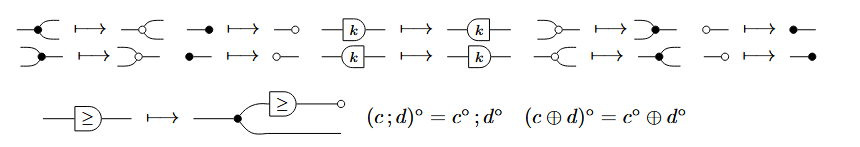
\includegraphics[width=1\linewidth]{images/GPA/PolarOperator.png}
	\end{figure}
	Its action on diagrams is defined functorially by
	$(a \circ b)^\circ = a^\circ \circ b^\circ$.
\end{definition}

\begin{proposition}[Second Normal Form]
	Every diagram $s \in \mathbf{GPA}_{\rtop}$ can be written as:
	\begin{figure}[H]
		\centering
		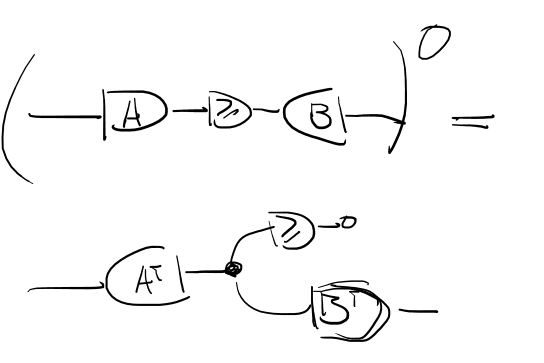
\includegraphics[width=.75\linewidth]{images/GPA/SecondNormalFormGPA.png}
	\end{figure}
\end{proposition}

\begin{proof}
	Apply the polar operator to the first normal form of every diagram
	$c \in \mathbf{GPA}_{\rtop}$. Since the polar operator is an
	involution and acts functorially, the result is again a valid diagram
	in $\mathbf{GPA}_{\rtop}$ in the claimed form.
\end{proof}

The second normal form expresses every diagram as a conic combination of
column vectors, which is precisely the $V$-representation of a polyhedral
cone. This is the representation that will drive the completeness proof:
two diagrams that are semantically equal must have the same conic hull,
and the axioms of $\mathbf{GPA}_{\rtop}$ are exactly sufficient to
witness this equality diagrammatically.

\section{Presentation results for \texorpdfstring{$\mathbf{PCRel}$}{PCRel}}

We now develop the presentation theory for the homogeneous case, proceeding
to establish the three properties that together yield the presentation of
$\mathbf{PCRel}$.

\begin{lemma}[Soundness]
	If $s = t$ in $\mathrm{FreeP}_{\mathbf{GPA}_{\rtop}}$, then
	$[s] = [t]$ in $\mathbf{PCRel}$.
\end{lemma}

\begin{proof}
	All axioms except those involving the newly introduced $\ge$
	generator are already present in $\mathbf{GAA}$ and therefore
	verified. It suffices to check that the new axioms preserve the
	semantics:
	\begin{figure}[H]
		\centering
		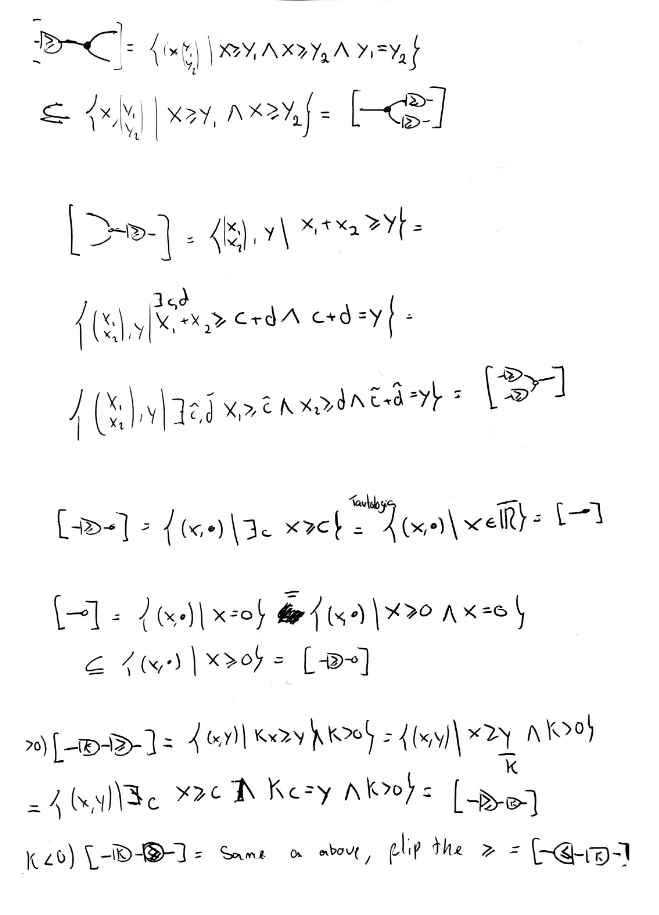
\includegraphics[width=1\linewidth]{images/GPA/SoundnessPCRel1.png}
	\end{figure}
	\begin{figure}[H]
		\centering
		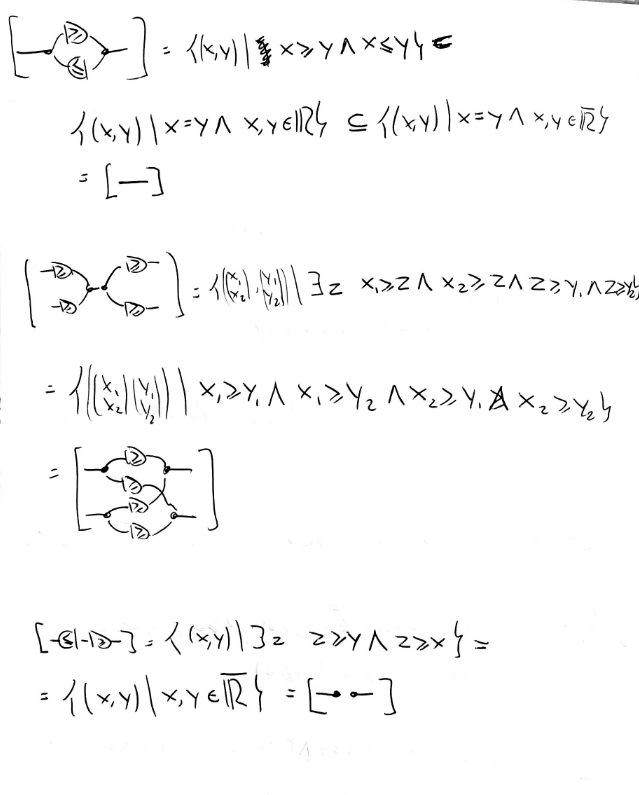
\includegraphics[width=1\linewidth]{images/GPA/SoundnessPCRel2.png}
	\end{figure}
\end{proof}

\begin{lemma}[Expressivity]
	For every $f : m \to n$ in $\mathbf{PCRel}$ there exists a
	$\Sigma$-term $s : m \to n$ in
	$\mathrm{Hom}_{\mathrm{FreeP}_{\mathbf{GPA}_{\rtop}}}(m,n)$
	such that $[s] = f$.
\end{lemma}

\begin{proof}
	By Definition~\ref{def:pcform}, every polyhedral cone has the form
	$\{x \mid Ax \ge 0,\ x \in \mathbb{R}^n\}$. This is precisely the
	interpretation of the diagram:
	\begin{figure}[H]
		\centering
		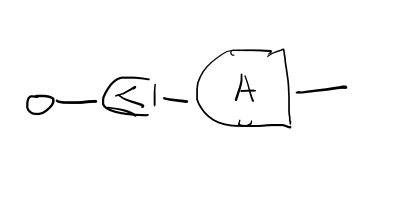
\includegraphics[width=.75\linewidth]{images/GPA/PCRelExpressivity.png}
	\end{figure}
\end{proof}

\begin{lemma}[Completeness]
	If $[s] = [t]$ in $\mathbf{PCRel}$, then $s = t$ in
	$\mathrm{FreeP}_{\mathbf{GPA}_{\rtop}}$.
\end{lemma}

\begin{proof}
	By the second normal form, we write $s$ and $t$ in
	$V$-representation form:
	\begin{figure}[H]
		\centering
		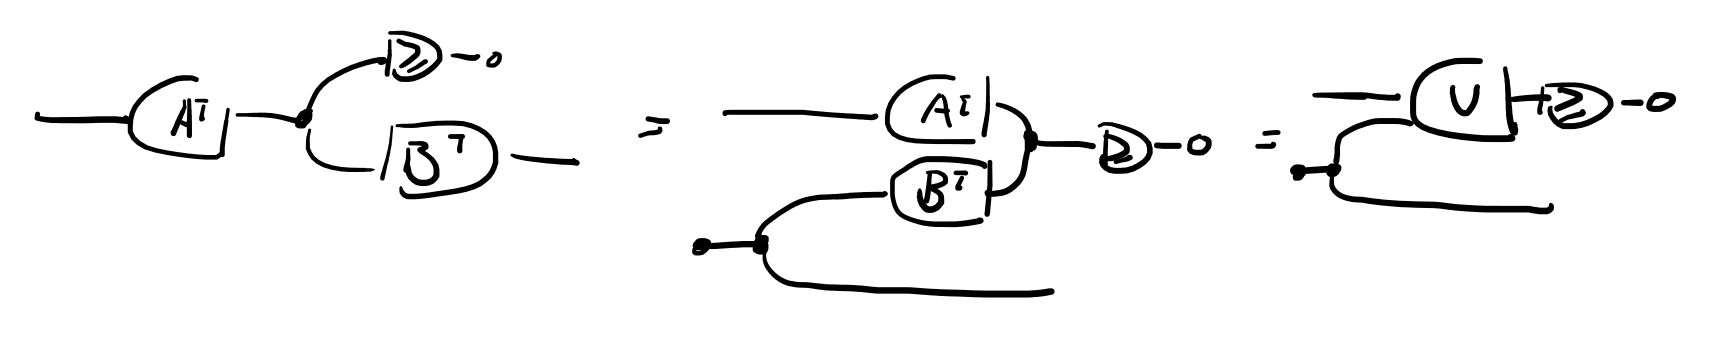
\includegraphics[width=1\linewidth]{images/GPA/ProofCompleteness1.png}
	\end{figure}
	The semantics of such a diagram is the conic hull of the column
	vectors of $V$. Since $[s] = [t]$ implies in particular
	$[s] \subseteq [t]$, the conic combinations of $V_t$ are a subset
	of those of $V_s$. Hence there exists a non-negative matrix $C$ such
	that $CV_t = V_s$. The diagrammatic witness is:
	\begin{figure}[H]
		\centering
		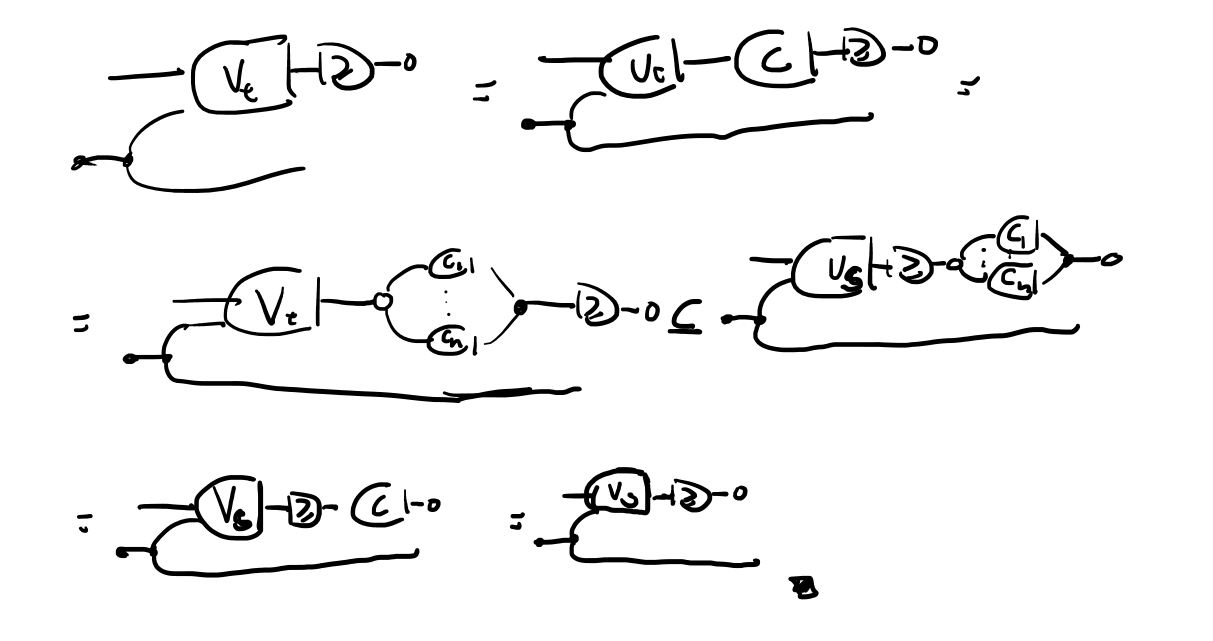
\includegraphics[width=1\linewidth]{images/GPA/ProofCompleteness2.png}
	\end{figure}
	The inclusion $[s] \subseteq [t]$ follows by the same argument,
	yielding equality.
\end{proof}

\begin{theorem}
	$\mathbf{PCRel}$ is presented by $\mathrm{FreeP}_{\mathbf{GPA}_{\rtop}}$.
\end{theorem}

\begin{proof}
	Soundness, expressivity, and completeness were established by the
	preceding three lemmas. Together they imply that the canonical PROP
	morphism is an isomorphism.
\end{proof}

This settles the homogeneous case: every polyhedral cone is diagrammatically
expressible, and two diagrams denote the same cone exactly when the axioms
can prove them equal. Cones are, however, a narrow class, they always
contain the origin, so they cannot represent an arbitrary feasible region
or, later, an arbitrary linear program. The next step lifts this result
from cones to general polyhedra, replacing the homogeneous inequalities
$Ax \ge 0$ with the affine $Ax \ge b$, and the machinery developed above
will carry over almost unchanged.

\section{Semantics: the prop \texorpdfstring{$\mathbf{PolyRel}$}{PolyRel}
  of polyhedra}
Now we start the presentation of the broader class of polyhedral relations by recalling the definition of a polyhedron.

\begin{definition}\label{polyform}
	A set $P \subseteq \mathbb{R}^n$ is called a \emph{polyhedron} if there
	exist $A \in \mathbb{R}^{m \times n}$ and $b \in \mathbb{R}^m$ such that
	\[
		P = \{x \in \mathbb{R}^n \mid Ax \ge b\}.
	\]
\end{definition}

Note that a polyhedral cone is a special case of a polyhedron with $b = 0$.
The distinction is algebraically significant: cones are closed under
non-negative scaling and admit a purely homogeneous representation, while
general polyhedra may be translated. This distinction is reflected in the
two graphical algebras we now define, where $\mathbf{GPA}_{\rtop}$ handles
the homogeneous case and $\mathbf{GPA}$ extends it with an affine generator.

In that light, one can define the category of polyhedral relations as:

\begin{definition}[The prop $\mathbf{PolyRel}$ of polyhedra]
	Let $k$ be an ordered field. The prop $\mathbf{PolyRel}_k$ is defined
	as follows:
	\begin{itemize}
		\item Objects are natural numbers $n \in \mathbb{N}$, interpreted
		      as the space $k^n$.
		\item A morphism $n \to m$ is a polyhedron
		      $R \subseteq k^n \times k^m$
		      for which there exist $p \in \mathbb{N}$,
		      $A \in k^{p \times (n+m)}$, and $b \in k^p$ such that
		      \[
			      R = \left\{ (x,y) \in k^n \times k^m \;\middle|\;
			      A \begin{pmatrix} x \\ y \end{pmatrix} + b \ge 0 \right\}.
		      \]
		\item Composition is relational composition.
		\item The monoidal product on objects is addition $n \otimes m := n+m$,
		      and on morphisms is the Cartesian product.
	\end{itemize}
\end{definition}

Notice how, the same way that \textbf{PCRel} offered us a more relational way to think about Polyhedral Cones, so does \textbf{PolyRel}.
Indeed, one may think of polyhedrals as closed spaces in some geometry that respects some linear constraints.
We argue, however, that this definition is overly convoluted, and a more natural way
to denote such objects is to think in terms of relations $R$,
such that $xRy \iff Ax + b \ge By +c$ for some matrices $A,B$ and  vectors $b,c$.
Once again, we move from a set-theoretic heavy description to a more logical one.

\section{Syntax: the algebra \texorpdfstring{$\mathbf{GPA}$}{GPA}}

We now extend the theory from polyhedral cones to general polyhedra by
reintroducing the affine generator $\rtop$. Geometrically, this
corresponds to allowing translations: a polyhedron is a translated
polyhedral cone, and the generator $\rtop$ provides the syntactic means
to encode the right-hand side vector $b$ in $Ax \ge b$. The normal form,
soundness, and expressivity arguments all extend smoothly from the
homogeneous case.

\begin{theorem}[Normal Form]\label{thm:normalformgpa}
	For every diagram $c$ in $\mathbf{GPA}$, there exists a diagram $d$
	such that $c = d$ modulo the axioms and $d$ is of the form:
	\begin{figure}[H]
		\centering
		\begin{tikzpicture}[axpic]
    \pic[val=A] (g1) at (0.500,0.500) {relation};
    \begin{scope}[shift={(1.250,0.000)}]
        \pic (g2) at (0.500,0.500) {ge};
    \end{scope}
    \draw (g1-out-0) to[out=0,in=180] (g2-in-0);
    \begin{scope}[shift={(2.500,0.000)}]
        \pic[val=B] (g3) at (0.500,0.500) {comatrix};
    \end{scope}
    \draw (g2-out-0) to[out=0,in=180] (g3-in-0);
\end{tikzpicture}

	\end{figure}
\end{theorem}

\begin{proof}
	The derivation proceeds directly. Let $c$ be a
	diagram of \textbf{GPA}. Then we can collect all $\rtop$ on the left such
	that $c'$ is a diagram of $\textbf{GPA}_{\rtop}$

	\begin{figure}[H]
		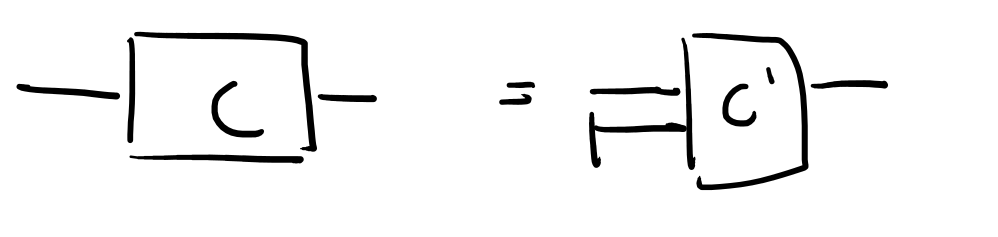
\includegraphics[width=1\linewidth]{images/GPA/affineGPAProof1.png}
	\end{figure}

	From Theorem~\ref{thm:FirstNormalForm} we know that $c'$ admits a normal form in
	terms of matrices A and B. Breaking down the matrix A in columns we get:

	\begin{figure}[H]
		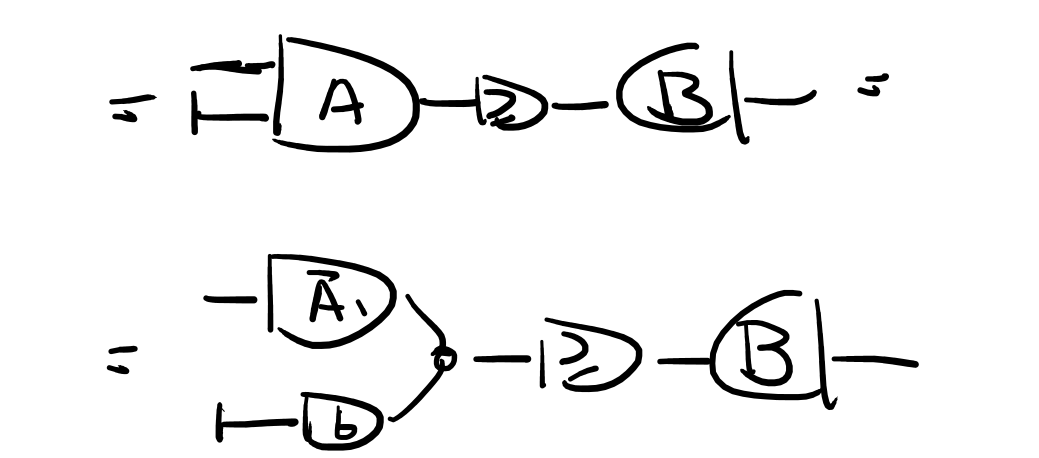
\includegraphics[width=1\linewidth]{images/GPA/affineGPAProof2.png}
	\end{figure}

	thus the thesis.
\end{proof}

\section{Presentation results for \texorpdfstring{$\mathbf{PolyRel}$}{PolyRel}}

\begin{lemma}[Soundness]
	If $s = t$ in $\mathrm{FreeP}_{\mathbf{GPA}}$, then $[s] = [t]$
	in $\mathbf{PolyRel}$.
\end{lemma}

\begin{proof}
	This follows immediately from the soundness of $\mathbf{PCRel}$.
	Since the generator $\rtop$ introduces no new axioms beyond those
	already verified for $\mathbf{PCRel}$ and $\mathbf{GAA}$, and both
	of those theories are sound in $\mathbf{PolyRel}$, soundness carries
	over directly.
\end{proof}

\begin{lemma}[Expressivity]
	For every $f : m \to n$ in $\mathbf{PolyRel}$ there exists a
	$\Sigma$-term $s : m \to n$ in
	$\mathrm{Hom}_{\mathrm{FreeP}_{\mathbf{GPA}}}(m,n)$
	such that $[s] = f$.
\end{lemma}

\begin{proof}
	By Definition~\ref{polyform}, every polyhedron has the form
	$\{x \mid Ax \ge b\}$. Appealing to this representation directly,
	the polyhedron is expressed as the interpretation of the following
	diagram, where the generator $\rtop$ encodes the right-hand side
	vector $b$:
	\begin{figure}[H]
		\centering
		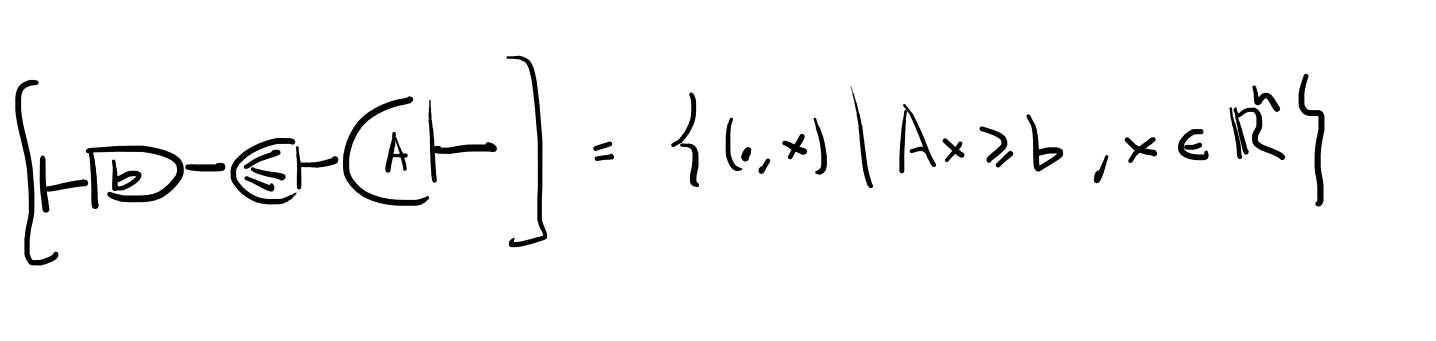
\includegraphics[width=1\linewidth]{images/GPA/ExpressivityPolyRel.png}
	\end{figure}
\end{proof}

\begin{lemma}[Completeness]
	If $[s] = [t]$ in $\mathbf{PolyRel}$, then $s = t$ in
	$\mathrm{FreeP}_{\mathbf{GPA}}$.
\end{lemma}

\begin{proof}
	Every polyhedron $P$ can be homogenised by introducing a slack variable,
	reducing the affine case to the conic one
	$P^H = \{(x,y) \in k^{n+1} | Ax + by \ge 0, y \ge 0\}$ which
	admits a normal form (Theorem~\ref{thm:FirstNormalForm}).
	Under this homogenisation, for each two diagrams $s, t \in \mathbf{GPA}$
	with $[s] = [t]$ in  $\mathbf{PolyRel}$, there are $s', t'$
	in $\mathbf{GPA}_{\rtop}$ such that $[s'] = [s]^H, [t'] = [t]^H $.
	Since two polyhedrals $P,Q$ are equal iff $P^H = Q^H$, then $s$ and
	$t$ have equal semantics in $\mathbf{PCRel}$.
	Completeness of $\mathbf{GPA}_{\rtop}$ then gives equality
	of the  homogenised diagrams, and de-homogenising recovers
	equality of $s$  and $t$ in $\mathrm{FreeP}_{\mathbf{GPA}}$.

	Diagrammatically this goes as follows:
	\begin{figure}[H]
		\centering
        \begin{tikzpicture}[axpic]
  \begin{scope}[shift={(0.625,1.000)}]
  \pic[val=A] (g1) at (0.500,0.500) {matrix};
  \end{scope}
  \pic (g2) at (0.500,0.500) {affine};
  \begin{scope}[shift={(1.250,0.000)}]
  \pic[val=b] (g3) at (0.500,0.500) {scalar};
  \end{scope}
  \draw (g2-out-0) to[out=0,in=180] (g3-in-0);
  \coordinate (a4) at (0.000,0 |- g1-in-0);
  \draw (g1-in-0) -- (a4);
  \coordinate (a5) at (2.250,0 |- g1-out-0);
  \draw (g1-out-0) -- (a5);
  \begin{scope}[shift={(2.500,0.500)}]
  \pic (g6) at (0.500,0.500) {multiplication};
  \end{scope}
  \draw (a5) to[out=0,in=180] (g6-in-0);
  \draw (g3-out-0) to[out=0,in=180] (g6-in-1);
  \begin{scope}[shift={(3.750,0.500)}]
  \pic (g7) at (0.500,0.500) {ge};
  \end{scope}
  \draw (g6-out-0) to[out=0,in=180] (g7-in-0);
  \begin{scope}[shift={(5.000,0.500)}]
  \pic[val=B] (g8) at (0.500,0.500) {comatrix};
  \end{scope}
  \draw (g7-out-0) to[out=0,in=180] (g8-in-0);
\end{tikzpicture}
\begin{tikzpicture}[axpic]\node{$=$};\end{tikzpicture}
\begin{tikzpicture}[axpic]
  \begin{scope}[shift={(0.000,1.000)}]
  \begin{scope}[shift={(0.625,1.000)}]
  \pic[val=A] (g1) at (0.500,0.500) {matrix};
  \end{scope}
  \pic (g2) at (0.500,0.500) {affine};
  \begin{scope}[shift={(1.250,0.000)}]
  \pic[val=b] (g3) at (0.500,0.500) {scalar};
  \end{scope}
  \draw (g2-out-0) to[out=0,in=180] (g3-in-0);
  \coordinate (a4) at (0.000,0 |- g1-in-0);
  \draw (g1-in-0) -- (a4);
  \coordinate (a5) at (2.250,0 |- g1-out-0);
  \draw (g1-out-0) -- (a5);
  \end{scope}
  \pic (g6) at (0.500,0.500) {affine};
  \begin{scope}[shift={(1.250,0.000)}]
  \pic (g7) at (0.500,0.500) {discard};
  \end{scope}
  \draw (g6-out-0) to[out=0,in=180] (g7-in-0);
  \begin{scope}[shift={(2.500,1.500)}]
  \pic (g8) at (0.500,0.500) {multiplication};
  \end{scope}
  \draw (a5) to[out=0,in=180] (g8-in-0);
  \draw (g3-out-0) to[out=0,in=180] (g8-in-1);
  \begin{scope}[shift={(3.750,1.500)}]
  \pic (g9) at (0.500,0.500) {ge};
  \end{scope}
  \draw (g8-out-0) to[out=0,in=180] (g9-in-0);
  \begin{scope}[shift={(5.000,1.500)}]
  \pic[val=B] (g10) at (0.500,0.500) {comatrix};
  \end{scope}
  \draw (g9-out-0) to[out=0,in=180] (g10-in-0);
\end{tikzpicture} \\
\vspace{3mm}

\;\begin{tikzpicture}[axpic]\node{$=$};\end{tikzpicture}\;
\begin{tikzpicture}[axpic]
  \begin{scope}[shift={(0.625,1.000)}]
  \begin{scope}[shift={(0.625,1.000)}]
  \pic[val=A] (g1) at (0.500,0.500) {matrix};
  \end{scope}
  \pic (g2) at (0.500,0.500) {affine};
  \begin{scope}[shift={(1.250,0.000)}]
  \pic[val=b] (g3) at (0.500,0.500) {scalar};
  \end{scope}
  \draw (g2-out-0) to[out=0,in=180] (g3-in-0);
  \coordinate (a4) at (0.000,0 |- g1-in-0);
  \draw (g1-in-0) -- (a4);
  \coordinate (a5) at (2.250,0 |- g1-out-0);
  \draw (g1-out-0) -- (a5);
  \end{scope}
  \pic (g6) at (0.500,0.500) {affine};
  \begin{scope}[shift={(1.250,0.000)}]
  \pic (g7) at (0.500,0.500) {ge};
  \end{scope}
  \draw (g6-out-0) to[out=0,in=180] (g7-in-0);
  \begin{scope}[shift={(2.500,0.000)}]
  \pic (g8) at (0.500,0.500) {discard};
  \end{scope}
  \draw (g7-out-0) to[out=0,in=180] (g8-in-0);
  \coordinate (a9) at (0.000,0 |- a4);
  \draw (a4) -- (a9);
  \coordinate (a10) at (3.500,0 |- a5);
  \draw (a5) -- (a10);
  \coordinate (a11) at (3.500,0 |- g3-out-0);
  \draw (g3-out-0) -- (a11);
  \begin{scope}[shift={(3.750,1.500)}]
  \pic (g12) at (0.500,0.500) {multiplication};
  \end{scope}
  \draw (a10) to[out=0,in=180] (g12-in-0);
  \draw (a11) to[out=0,in=180] (g12-in-1);
  \begin{scope}[shift={(5.000,1.500)}]
  \pic (g13) at (0.500,0.500) {ge};
  \end{scope}
  \draw (g12-out-0) to[out=0,in=180] (g13-in-0);
  \begin{scope}[shift={(6.250,1.500)}]
  \pic[val=B] (g14) at (0.500,0.500) {comatrix};
  \end{scope}
  \draw (g13-out-0) to[out=0,in=180] (g14-in-0);
\end{tikzpicture}
\begin{tikzpicture}[axpic]\node{$=$};\end{tikzpicture}
\vspace{5mm}

\begin{tikzpicture}[axpic]\node{$=$};\end{tikzpicture}
\begin{tikzpicture}[axpic]
  \begin{scope}[shift={(0.000,0.500)}]
  \begin{scope}[shift={(0.625,1.500)}]
  \coordinate (id_in_1) at (0,0.500);
  \coordinate (id_out_2) at (1.000,0.500);
  \draw (id_in_1) -- (id_out_2);
  \end{scope}
  \pic (g3) at (0.500,0.500) {affine};
  \begin{scope}[shift={(1.250,0.000)}]
  \pic (g4) at (0.500,0.500) {copy};
  \end{scope}
  \draw (g3-out-0) to[out=0,in=180] (g4-in-0);
  \coordinate (a5) at (0.000,0 |- id_in_1);
  \draw (id_in_1) -- (a5);
  \coordinate (a6) at (2.250,0 |- id_out_2);
  \draw (id_out_2) -- (a6);
  \end{scope}
  \begin{scope}[shift={(2.500,0.000)}]
  \begin{scope}[shift={(0.000,1.000)}]
  \begin{scope}[shift={(0.000,1.000)}]
  \pic[val=A] (g7) at (0.500,0.500) {matrix};
  \end{scope}
  \pic[val=b] (g8) at (0.500,0.500) {scalar};
  \end{scope}
  \pic (g9) at (0.500,0.500) {ge};
  \end{scope}
  \draw (a6) to[out=0,in=180] (g7-in-0);
  \draw (g4-out-0) to[out=0,in=180] (g8-in-0);
  \draw (g4-out-1) to[out=0,in=180] (g9-in-0);
  \begin{scope}[shift={(3.750,0.500)}]
  \begin{scope}[shift={(0.000,1.000)}]
  \pic (g10) at (0.500,0.500) {multiplication};
  \end{scope}
  \pic (g11) at (0.500,0.000) {cozero};
  \end{scope}
  \draw (g7-out-0) to[out=0,in=180] (g10-in-0);
  \draw (g8-out-0) to[out=0,in=180] (g10-in-1);
  \draw (g9-out-0) to[out=0,in=180] (g11-in-0);
  \begin{scope}[shift={(5.000,1.500)}]
  \pic (g12) at (0.500,0.500) {ge};
  \end{scope}
  \draw (g10-out-0) to[out=0,in=180] (g12-in-0);
  \begin{scope}[shift={(6.250,1.500)}]
  \pic[val=B] (g13) at (0.500,0.500) {comatrix};
  \end{scope}
  \draw (g12-out-0) to[out=0,in=180] (g13-in-0);
\end{tikzpicture}

	\end{figure}

	Whereas the interpretation of the last diagram is
	$\{(x,y,z) \in k^m | Ax + by \ge Bz, y \ge 0\}$, which is the same
	as $P^H$. Therefore, the semantics of $s'$ is that of the homogenisation
	of $[s]$ and follows the above argument.
\end{proof}

\begin{theorem}
	$\mathbf{PolyRel}$ is presented by $\mathrm{FreeP}_{\mathbf{GPA}}$.
\end{theorem}

\begin{proof}
	By the preceding three lemmas.
\end{proof}

This is the result the rest of the thesis leans on: every polyhedral
relation, not just the conic ones from earlier, has a diagrammatic
representative, and semantic equality between polyhedra can always be
certified by a finite rewriting sequence in $\mathbf{GPA}$. It is this
presentation, together with its normal form, that
Chapter~\ref{sec:glp} builds on when it adds a single new generator for
the objective function.

\begin{remark}[Invariance under non-negative matrices]
	Whereas the linearity axiom shows the linear generator to be exactly
	invariant under column-stochastic reweightings (Remark~\ref{rmk:stochastic}),
	the order generator $\mathrm{ge}$ enjoys a related but weaker property with
	respect to non-negative matrices. Let $A \in \mathbb{R}^{n \times m}$ with
	$A_{ij} \ge 0$ for all $i,j$. If $x, y \in \mathbb{R}^m$ satisfy $x \ge y$
	componentwise, then $Ax \ge Ay$ componentwise: for each row $i$,
	\[
		(Ax)_i - (Ay)_i = \sum_{j} A_{ij}(x_j - y_j) \ge 0,
	\]
	since every term is a product of a non-negative entry and a non-negative
	difference. Diagrammatically, this is the inclusion
	\[
		\mathrm{matrix}[A] \; ; \; \mathrm{ge}^{\otimes n}
		\;\subseteq\;
		\mathrm{ge}^{\otimes m} \; ; \; \mathrm{matrix}[A]^{\otimes 2},
	\]
	verified directly in the semantics of $\mathbf{PolyRel}$, exactly as the
	axioms of $\mathbf{GPA}$ are themselves verified. Unlike
	Remark~\ref{rmk:stochastic}, this is only an inclusion and not an equality:
	a non-negative matrix need not reflect the order, only preserve it, so
	$Ax \ge Ay$ can hold even when $x \ge y$ fails (take $A = 0$). In other
	words, a non-negative matrix always goes through the order generator,
	certifying that any inequality derived in $\mathbf{GPA}$ remains valid
	after left multiplication by $A$.
\end{remark}
